% =====================================================================
%  Thesis — Dimitrios Karagiannis
%  Sequential and Parallel Algorithms
%  Compatible with pdfLaTeX
% =====================================================================


% ---------------- PACKAGES ----------------
\documentclass[12pt,a4paper]{article}

% PACKAGES
\usepackage[LGR,T1]{fontenc}
\usepackage[utf8]{inputenc}
\usepackage[english,greek]{babel}


\usepackage{graphicx}
\usepackage{booktabs}
\usepackage{listings}
\usepackage{enumerate}
\usepackage{amssymb}
\usepackage{amsmath}
\usepackage{xcolor}
\usepackage{float}
\usepackage{afterpage}
\usepackage{geometry}
\geometry{margin=2.5cm}

\usepackage{hyperref}
\hypersetup{colorlinks=true, linkcolor=black}

% ALGORITHMS
\usepackage{algorithm}
\usepackage{algpseudocode}
\usepackage{caption}

% TIKZ
\usepackage{tikz}
\usetikzlibrary{positioning,shapes,arrows.meta}

\tikzset{
    vertex/.style={circle, draw, fill=blue!20, minimum size=8mm, font=\small},
    edge weight/.style={font=\small, inner sep=1pt, fill=white, text=black}
}

% TABLES
\usepackage{array}
\usepackage[table]{xcolor}

% PLOTS
\usepackage{pgfplots}
\pgfplotsset{compat=1.17}

% BIBLIOGRAPHY
\usepackage{csquotes}
\usepackage[backend=biber,style=numeric,sorting=none]{biblatex}
\addbibresource{references.bib}



% ---------------- HYPERREF SETTINGS ----------------
\hypersetup{
    colorlinks=true,
    linkcolor=black,
    filecolor=magenta,
    urlcolor=cyan,
}


\usepackage{array}
\usepackage[table]{xcolor}
\usepackage[backend=biber,style=numeric,sorting=none]{biblatex}
\addbibresource{references.bib}



% =====================================================================
%  DOCUMENT INFO
% =====================================================================
\title{Σειριακοί και Παράλληλοι Αλγόριθμοι\\[4pt]
\large \foreignlanguage{english}{Sequential and Parallel Algorithms}}
\author{Καραγιάννης Δημήτριος \\ 1115202200293 \\ \texttt{sdi2200293@di.uoa.gr}}
\date{Καλοκαίρι 2026}

% =====================================================================
\begin{document}

% ---------------- COVER PAGE ----------------
\thispagestyle{empty}
\begin{center}

\includegraphics[width=0.15\textwidth]{ekpa_logo.jpg}\\[0.5cm]

\textbf{\Large Εθνικό και Καποδιστριακό Πανεπιστήμιο Αθηνών}\\[0.3cm]
\textbf{\large Τμήμα Πληροφορικής και Τηλεπικοινωνιών}\\[3cm]

{\Large \textbf{Πτυχιακή Εργασία}}\\[0.5cm]
{\large \textbf{Σειριακοί και Παράλληλοι Αλγόριθμοι}}\\[3cm]

\textbf{Καραγιάννης Δημήτριος}\\[0.2cm]
1115202200293\\[0.2cm]
\texttt{\foreignlanguage{english}{sdi2200293@di.uoa.gr}}\\[3cm]

Επιβλέπων Καθηγητής: \textbf{ΕΔΙΠ Δρ. Λουκά Μαρία}\\[1.5cm]

\vfill
{\large Καλοκαίρι 2026}\\[0.3cm]
\end{center}
\clearpage

\tableofcontents
\clearpage

% ---------------- BODY ----------------
\section*{Εισαγωγή}
\addcontentsline{toc}{section}{Εισαγωγή}
Σύντομη εισαγωγή... \nocite{*}
\clearpage

\section{Αλγόριθμοι Γραφημάτων}
Η θεωρία γραφημάτων διαδραματίζει σημαντικό ρόλο στην επιστήμη των υπολογιστών, επειδή παρέχει έναν εύκολο και συστηματικό τρόπο για τη μοντελοποίηση πολλών προβλημάτων. Πολλά προβλήματα μπορούν να εκφραστούν με όρους γραφημάτων και να επιλυθούν με τη χρήση τυπικών αλγορίθμων γραφημάτων. Το παρόν κεφάλαιο παρουσιάζει παράλληλες υλοποιήσεις κάποιων σημαντικών και θεμελιωδών αλγορίθμων γραφημάτων.


\subsection{Ορισμοί και Αναπαράσταση}
Ένα μη κατευθυνόμενο γράφημα $G$ είναι ένα ζεύγος $(V, E)$, όπου $V$ είναι ένα πεπερασμένο σύνολο σημείων που ονομάζονται κορυφές και $E$ είναι
ένα πεπερασμένο σύνολο ακμών. Μια ακμή $e \in E$
 είναι ένα μη διατεταγμένο ζεύγος $(u, v)$, όπου $(u, v) \in V$. Μια ακμή $(u, v)$
υποδηλώνει ότι οι κορυφές $u$ και $v$ είναι συνδεδεμένες. Ομοίως, ένα κατευθυνόμενο γράφημα $G$ είναι ένα ζεύγος $(V, E)$,
όπου $V$ είναι το σύνολο των κορυφών όπως μόλις ορίσαμε, αλλά μια ακμή $(u, v) \in E$ είναι ένα διατεταγμένο ζεύγος, δηλαδή
υποδηλώνει ότι υπάρχει σύνδεση από το $u$ στο $v$. Το Σχήμα ~\ref{fig:graph1} απεικονίζει ένα μη κατευθυνόμενο και ένα
κατευθυνόμενο γράφημα. Χρησιμοποιούμε τον όρο γράφημα για να αναφερθούμε τόσο στα κατευθυνόμενα όσο και στα μη κατευθυνόμενα γραφήματα.

Πολλοί ορισμοί είναι κοινοί για κατευθυνόμενα και μη κατευθυνόμενα γραφήματα, αν και ορισμένοι όροι έχουν ελαφρώς διαφορετική σημασία στο καθένα.
Αν η $(u, v)$ είναι μια ακμή σε ένα μη κατευθυνόμενο γράφημα, τότε η $(u, v)$ συνδέει (\textbf{\foreignlanguage{english}{incident on}}) τις κορυφές $u$ και $v$.
Ωστόσο, αν το γράφημα είναι κατευθυνόμενο, τότε η ακμή $(u, v)$ ξεκινάει (\textbf{\foreignlanguage{english}{incident from}}) από την κορυφή $u$ και καταλήγει (\textbf{\foreignlanguage{english}{incident to}}) στην κορυφή $v$.
Για παράδειγμα, στο Σχήμα ~\ref{fig:graph1}(α), η ακμή $e$ συνδέει (\textbf{\foreignlanguage{english}{incident on}}) τις κορυφές 5 και 4, ενώ στο Σχήμα ~\ref{fig:graph1}(β), η ακμή $f$ ξεκινάει (\textbf{\foreignlanguage{english}{incident from}}) από την κορυφή 5 και καταλήγει (\textbf{\foreignlanguage{english}{incident to}}) στην κορυφή 2.
Αν η $(u, v)$ είναι μια ακμή σε έναν μη κατευθυνόμενο γράφημα $G = (V, E)$, οι κορυφές $u$ και $v$ λέγεται ότι είναι γειτονικές (\textbf{\foreignlanguage{english}{adjacent}}) μεταξύ τους.
Αν το γράφημα είναι κατευθυνόμενο, η κορυφή $v$ λέγεται ότι είναι γειτονική της (\textbf{\foreignlanguage{english}{adjacent to}}) κορυφής $u$.



\begin{figure}[ht]
\centering

\begin{minipage}{0.45\textwidth}
\centering
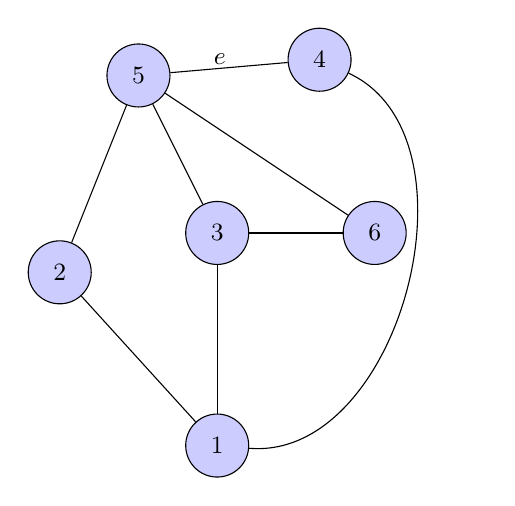
\begin{tikzpicture}[scale=1.0, every node/.style={transform shape}]
    \node[vertex] (5) at (0,2) {5};
    \node[vertex] (2) at (-1,-0.5) {2};
    \node[vertex] (3) at (1,0) {3}; 
    \node[vertex] (1) at (1,-2.7) {1};
    \node[vertex] (6) at (3,0) {6};
    \node[vertex] (4) at (2.3,2.2) {4};

    \draw (5) -- (2);
    \draw (5) -- (3); 
    \draw (5) -- (4) node[midway, above left, edge weight] {$e$};
    \draw (2) -- (1); 
    \draw (3) -- (1); 
    \draw (3) -- (6); 
    \draw (5) -- (6); 
    \draw[bend left=80] (4) to (1);

\end{tikzpicture}
\end{minipage}
\hfill
\begin{minipage}{0.45\textwidth}
\centering
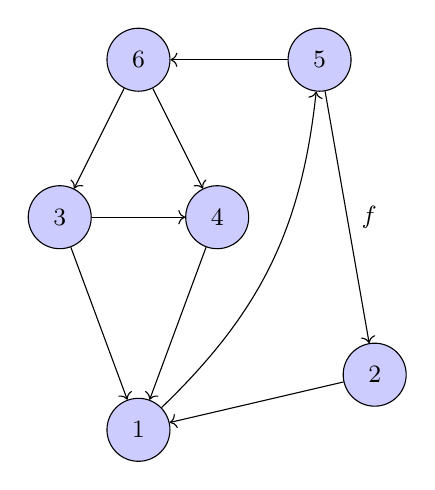
\begin{tikzpicture}[scale=1.0, every node/.style={transform shape}]
    \node[vertex] (6) at (0,2) {6};
    \node[vertex] (3) at (-1,0) {3};
    \node[vertex] (4) at (1,0) {4}; 
    \node[vertex] (1) at (0,-2.7) {1};
    \node[vertex] (2) at (3,-2) {2};
    \node[vertex] (5) at (2.3,2) {5};

    \draw[->] (6) -- (3);
    \draw[->] (6) -- (4);
    \draw[->] (3) -- (4);
    \draw[->] (3) -- (1);
    \draw[->] (4) -- (1);
    \draw[bend right=20, ->] (1) to (5);
    \draw[->] (5) -- (6);
    \draw[->] (5) -- (2) node[midway, right, xshift=4pt, edge weight] {$f$};
    \draw[->] (2) -- (1);

\end{tikzpicture}
\end{minipage}

\vspace{0.3cm}
\noindent\rule{\textwidth}{0.2pt}
\caption{(a) Ένα μη κατευθυνόμενο γράφημα και (b) ένα κατευθυνόμενο γράφημα.}
\label{fig:graph1}
\end{figure}
\vspace{0.5cm}

\begin{figure}[ht]
\centering

\begin{minipage}{0.45\textwidth}
\centering
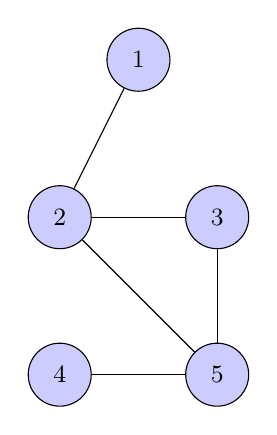
\begin{tikzpicture}[scale=1.0, every node/.style={transform shape}]
    \node[vertex] (1) at (1,2) {1};
    \node[vertex] (2) at (0,0) {2};
    \node[vertex] (3) at (2,0) {3}; 
    \node[vertex] (4) at (0,-2) {4};
    \node[vertex] (5) at (2,-2) {5};

    \draw (1) -- (2);
    \draw (2) -- (3); 
    \draw (2) -- (5); 
    \draw (3) -- (5); 
    \draw (5) -- (4); 

 
\end{tikzpicture}
\end{minipage}
\hfill
\begin{minipage}{0.45\textwidth}
\centering
\[
A =
\begin{bmatrix}
0 & 1 & 0 & 0 & 0 \\
1 & 0 & 1 & 0 & 1 \\
0 & 1 & 0 & 0 & 1 \\
0 & 0 & 0 & 0 & 1 \\
0 & 1 & 1 & 1 & 0 
\end{bmatrix}
\]

\end{minipage}

\vspace{0.3cm}
\noindent\rule{\textwidth}{0.2pt}
\caption{Ένα μη κατευθυνόμενο γράφημα και η αναπαράσταση του με λίστα γειτνίασης.}
\label{fig:graph2}
\end{figure}
\vspace{0.5cm}


Μια διαδρομή (ή μονοπάτι) από μια κορυφή $v$ σε μια κορυφή $u$ είναι μια ακολουθία $<v_0, v_1, v_2, ..., v_k>$ κορυφών, όπου $v_0$ = $v$, $v_k$ = $u$, και $(v_i, v_{i+1}) \in E$ για $i = 0, 1, ..., k-1$. Το μήκος μιας διαδρομής ορίζεται ως το πλήθος των ακμών σε αυτή τη διαδρομή. Αν υπάρχει διαδρομή από το $v$ στο $u$, τότε το $u$ είναι προσπελάσιμο (\textbf{\foreignlanguage{english}{reachable}}) από το $v$. Μια διαδρομή είναι απλή αν όλες οι κορυφές της είναι διακριτές (δεν επαναλαμβάνονται). Μια διαδρομή σχηματίζει κύκλο αν η αρχική και η τελική της κορυφή ταυτίζονται – δηλαδή, αν $v_0$ = $v_k$. Ένα γράφημα χωρίς κύκλους ονομάζεται ακυκλικό. Ένας κύκλος είναι απλός αν όλες οι ενδιάμεσες κορυφές του είναι διακριτές.


Για παράδειγμα, στο Σχήμα ~\ref{fig:graph1}(a), η ακολουθία $<3, 6, 5, 4>$ είναι μια διαδρομή από την κορυφή 3 στην κορυφή 4. Στο Σχήμα ~\ref{fig:graph1}(β), υπάρχει ένας κατευθυνόμενος απλός κύκλος $<1, 5, 6, 4, 1>$. Επίσης, στο Σχήμα ~\ref{fig:graph1}(α), η ακολουθία $<1, 2, 5, 3, 6, 5, 4, 1>$ είναι ένας μη κατευθυνόμενος κύκλος που δεν είναι απλός, γιατί περιέχει τον βρόχο $<5, 3, 6, 5>$.

Ένα μη κατευθυνόμενο γράφημα είναι συνεκτικό αν κάθε ζεύγος κορυφών ενώνεται με μια διαδρομή. Λέμε ότι ένα γράφημα $G' = (V', E')$ είναι υπογράφημα του $G = (V, E)$ αν $V'\subseteq V$ και $E'\subseteq E$. Για ένα δεδομένο σύνολο $V'\subseteq V$, το υπόγράφημα του $G$ που προκύπτει από το $V'$ είναι το γράφημα $G' = (V', E')$, όπου $E' = \{ (u, v) \in E \mid u, v \in V' \}$. Ένα πλήρες γράφημα είναι ένα γράφημα στον οποίο κάθε ζεύγος κορυφών είναι γειτονικό. Ένα δάσος είναι ένα ακυκλικό γράφημα και ένα δέντρο είναι ένα συνεκτικό ακυκλικό γράφημα. Σημειώστε ότι αν $G = (V, E)$ είναι ένα δέντρο, τότε $|E| = |V| - 1$.

Μερικές φορές τα βάρη συσχετίζονται με κάθε ακμή στο Ε. Τα βάρη είναι συνήθως πραγματικοί αριθμοί που αντιπροσωπεύουν το κόστος ή το όφελος της διαδρομής κατά μήκος της συνδεδεμένης ακμής. Για παράδειγμα, σε ένα ηλεκτρονικό κύκλωμα, μια αντίσταση μπορεί να αναπαρασταθεί από μια ακμή της οποίας το βάρος είναι η τιμή της  αντίστασής της. Ένα γράφημα που έχει βάρη συσχετισμένα με κάθε ακμή ονομάζεται γράφημα με βάρη και συμβολίζεται ως $G = (V, E, w)$, όπου τα $V$ και $E$ είναι όπως ορίσαμε προηγουμένως και η $w : E \to \mathbb{R}$ είναι μια πραγματική συνάρτηση που ορίζεται στο E. Το βάρος ενός γραφήματος ορίζεται ως το άθροισμα των βαρών των ακμών του. Το βάρος μιας διαδρομής είναι το άθροισμα των βαρών των ακμών της.

Υπάρχουν δύο τυπικές μέθοδοι για την αναπαράσταση ενός γραφήματος σε ένα πρόγραμμα υπολογιστή. Η πρώτη μέθοδος είναι η χρήση πίνακα (μήτρας), και η δεύτερη μέθοδος είναι η χρήση συνδεδεμένης λίστας.

Θεωρήστε ένα γράφημα $G = (V, E)$ με $n$ κορυφές αριθμημένες ως 1, 2, ..., $n$. Ο πίνακας γειτνίασης αυτού του γραφήματος είναι ένας $n \times n$ πίνακας $A = (a_{i,j})$, ο οποίος ορίζεται ως εξής: \[
a_{i,j} =
\begin{cases}
1 & \text{εάν } (v_i, v_j) \in E\\[2mm]
0 & \text{διαφορετικά}
\end{cases}
\]

Το Σχήμα ~\ref{fig:graph2} απεικονίζει μια αναπαράσταση με πίνακα γειτνίασης για έναν μη κατευθυνόμενο γράφημα. Σημειώστε ότι ο πίνακας γειτνίασης ενός μη κατευθυνόμενου γραφήματος είναι συμμετρικός. Η αναπαράσταση με πίνακα γειτνίασης μπορεί να τροποποιηθεί για να υποστηρίξει γραφήματα με βάρη. Σε αυτή την περίπτωση, ο $A = (a_{i,j})$ ορίζεται ως εξής:
\[
a_{i,j} =
\begin{cases}
w(v_i, v_j) & \text{εάν } (v_i, v_j) \in E\\[2mm]
0 & \text{εάν } i = j\\[2mm]
\infty & \text{διαφορετικά}
\end{cases}
\]




Αναφερόμαστε σε αυτόν τον τροποποιημένο πίνακα γειτνίασης ως πίνακα γειτνίασης με βάρη. Ο χώρος που απαιτείται για την αποθήκευση του πίνακα γειτνίασης ενός γραφήματος με $n$ κορυφές είναι $\Theta(n^2)$.

Η αναπαράσταση με λίστα γειτνίασης ενός γραφήματος $G = (V, E)$ αποτελείται από έναν πίνακα $Adj[1..|V|]$ λιστών. Για κάθε $v \in V$, η $Adj[v]$ είναι μια συνδεδεμένη λίστα όλων των κορυφών $u$ για τις οποίες ο $G$ περιέχει μια ακμή $(v, u) \in E$. Με άλλα λόγια, η $Adj[v]$ είναι μια λίστα όλων των κορυφών που είναι γειτονικές προς την $v$. Το Σχήμα ~\ref{fig:graph3} δείχνει ένα παράδειγμα αναπαράστασης με λίστα γειτνίασης. Η αναπαράσταση με λίστα γειτνίασης μπορεί να τροποποιηθεί για να φιλοξενήσει γραφήματα με βάρη,  αποθηκεύοντας το βάρος κάθε ακμής $(v, u) \in E$ στη λίστα γειτνίασης της κορυφής $v$. Ο χώρος που απαιτείται για την αποθήκευση της λίστας γειτνίασης είναι $\Theta(|E|)$.

\begin{figure}[ht]
\centering

\begin{minipage}{0.45\textwidth}
\centering
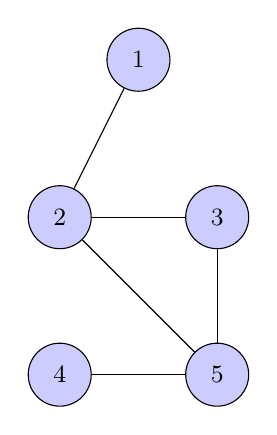
\begin{tikzpicture}[scale=1.0, every node/.style={transform shape}]
    \node[vertex] (1) at (1,2) {1};
    \node[vertex] (2) at (0,0) {2};
    \node[vertex] (3) at (2,0) {3}; 
    \node[vertex] (4) at (0,-2) {4};
    \node[vertex] (5) at (2,-2) {5};

    \draw (1) -- (2);
    \draw (2) -- (3); 
    \draw (2) -- (5); 
    \draw (3) -- (5); 
    \draw (5) -- (4); 

 
\end{tikzpicture}
\end{minipage}
\begin{minipage}{0.45\textwidth}
\centering
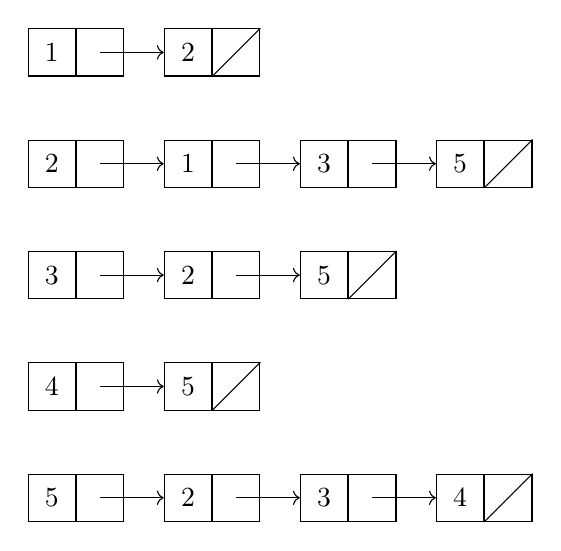
\begin{tikzpicture}[node distance=0.8cm, every node/.style={minimum width=0.6cm, minimum height=0.6cm, draw, align=center}]
    % Λίστα 1
    \node (a1) {1};
    \node (a2) [right=0cm of a1] {}; % δεξί κουτί χωρίς περιεχόμενο
    \node (a3) [right=0.5cm of a2] {2};
    \node (a4) [right=0cm of a3] {}; % δεξί κουτί χωρίς περιεχόμενο
    \draw (a4.north east) -- (a4.south west);
    \draw[->] (a2.center) -- (a3.west);
    
    % Λίστα 2
    \node (b1) [below=0.8cm of a1] {2};
    \node (b2) [right=0cm of b1] {};
    \node (b3) [right=0.5cm of b2] {1};
    \node (b4) [right=0cm of b3] {};
    \draw[->] (b2.center) -- (b3.west);
    \node (b5) [right=0.5cm of b4] {3};
    \node (b6) [right=0cm of b5] {};
    \draw[->] (b4.center) -- (b5.west);
    \node (b7) [right=0.5cm of b6] {5};
    \node (b8) [right=0cm of b7] {};
    \draw[->] (b6.center) -- (b7.west);
    \draw (b8.north east) -- (b8.south west);
    % διαγώνιος επειδή δεν υπάρχει επόμενο στοιχείο της λίστας


    % Λίστα 3
    \node (c1) [below=0.8cm of b1] {3};
    \node (c2) [right=0cm of c1] {};
    \node (c3) [right=0.5cm of c2] {2};
    \node (c4) [right=0cm of c3] {};
    \draw[->] (c2.center) -- (c3.west);
    \node (c5) [right=0.5cm of c4] {5};
    \node (c6) [right=0cm of c5] {};
    \draw[->] (c4.center) -- (c5.west);
    \draw (c6.north east) -- (c6.south west);
    
 

    % Λίστα 4
    \node (d1) [below=0.8cm of c1] {4};
    \node (d2) [right=0cm of d1] {}; % δεξί κουτί χωρίς περιεχόμενο
    \node (d3) [right=0.5cm of d2] {5};
    \node (d4) [right=0cm of d3] {}; % δεξί κουτί χωρίς περιεχόμενο
    \draw (d4.north east) -- (d4.south west);
    \draw[->] (d2.center) -- (d3.west);

    % Λίστα 5
    \node (e1) [below=0.8cm of d1] {5};
    \node (e2) [right=0cm of e1] {};
    \node (e3) [right=0.5cm of e2] {2};
    \node (e4) [right=0cm of e3] {};
    \draw[->] (e2.center) -- (e3.west);
    \node (e5) [right=0.5cm of e4] {3};
    \node (e6) [right=0cm of e5] {};
    \draw[->] (e4.center) -- (e5.west);
    \node (e7) [right=0.5cm of e6] {4};
    \node (e8) [right=0cm of e7] {};
    \draw[->] (e6.center) -- (e7.west);
    \draw (e8.north east) -- (e8.south west);
\end{tikzpicture}

\end{minipage}

\vspace{0.3cm}
\noindent\rule{\textwidth}{0.2pt}
\caption{Ένα μη κατευθυνόμενο γράφημα και η αναπαράσταση του με λίστα γειτνίασης.}
\label{fig:graph3}
\end{figure}
\vspace{2cm}


Η φύση του γραφήματος καθορίζει ποια αναπαράσταση πρέπει να χρησιμοποιηθεί. Ένα γράφημα $G = (V, E)$ είναι αραιό αν το $|E|$ είναι πολύ μικρότερο από $O(|V|^2)$, διαφορετικά είναι πυκνό. Η αναπαράσταση με πίνακα γειτνίασης είναι χρήσιμη για πυκνά γραφήματα, ενώ η αναπαράσταση με λίστα γειτνίασης είναι συχνά πιο αποδοτική για αραιά γραφήματα. Να σημειωθεί ότι ο ακολουθιακός χρόνος εκτέλεσης ενός αλγορίθμου που χρησιμοποιεί πίνακα γειτνίασης και χρειάζεται να διατρέξει όλες τις ακμές του γραφήματος είναι κάτω φραγμένος από $\Omega(|V|^2)$, επειδή πρέπει να προσπελαστεί ολόκληρος ο πίνακας. Ωστόσο, αν χρησιμοποιείται αναπαράσταση με λίστα γειτνίασης, ο χρόνος εκτέλεσης είναι κάτω φραγμένος από $\Omega(|V| + |E|)$ για τον ίδιο λόγο. Επομένως, αν το γράφημα είναι αραιό (το $|E|$ είναι πολύ μικρότερο από $|V|^2$), η αναπαράσταση με λίστα γειτνίασης είναι καλύτερη από την αναπαράσταση με πίνακα γειτνίασης.

Το υπόλοιπο αυτού του κεφαλαίου παρουσιάζει διάφορους αλγορίθμους γραφημάτων. Τα πρώτα τέσσερα εδάφια παρουσιάζουν αλγορίθμους για πυκνά γραφήματα, και το τελευταίο εδάφιο συζητά αλγορίθμους για αραιά γραφήματα. Υποθέτουμε ότι τα πυκνά γραφήματα αναπαρίστανται με έναν πίνακα γειτνίασης και αραιά γραφήματα με μια λίστα γειτνίασης. Σε όλο αυτό το κεφάλαιο, το n συμβολίζει τον αριθμό των κορυφών στο γράφημα.
\vspace{1cm}


\section{Eλάχιστο δέντρο επικάλυψης: Ο αλγόριθμος του \foreignlanguage{english}{Prim}}


\begin{figure}[ht]
\centering

\begin{minipage}{0.45\textwidth}
\centering
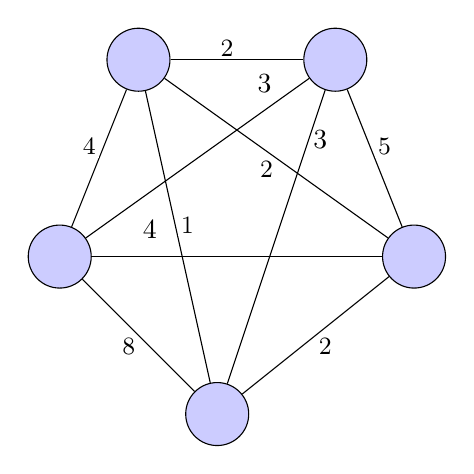
\begin{tikzpicture}[scale=1.0, every node/.style={transform shape}]
    \node[vertex] (5) at (0,2) {};
    \node[vertex] (2) at (-1,-0.5) {};
    \node[vertex] (1) at (1,-2.5) {};
    \node[vertex] (3) at (3.5,-0.5) {};
    \node[vertex] (4) at (2.5,2) {};

    \draw (5) -- (2) node[midway, above left, edge weight] {4};
    \draw (5) -- (3) node[midway, below left, edge weight] {2}; 
    \draw (5) -- (4) node[midway, above left, edge weight] {2};
    \draw (2) -- (1) node[midway, below left, edge weight] {8};
    \draw (3) -- (1) node[midway, below right, edge weight] {2};
    \draw (3) -- (4) node[midway, above right, edge weight] {5};
    \draw (2) -- (4) node[pos=0.8, above=1mm] {3};
    \draw (1) -- (4) node[pos=0.95, below=2mm] {3};
    \draw (2) -- (3) node[pos=0.2, above=1mm] {4};
    \draw (5) -- (1) node[midway, above right, edge weight] {1};


\end{tikzpicture}
\end{minipage}
\hfill
\begin{minipage}{0.45\textwidth}
\centering
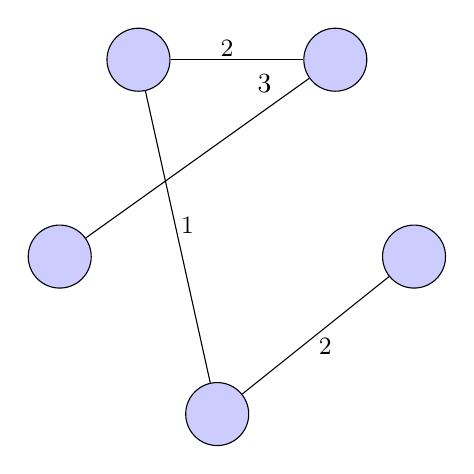
\begin{tikzpicture}[scale=1.0, every node/.style={transform shape}]
    \node[vertex] (5) at (0,2) {};
    \node[vertex] (2) at (-1,-0.5) {};
    \node[vertex] (1) at (1,-2.5) {};
    \node[vertex] (3) at (3.5,-0.5) {};
    \node[vertex] (4) at (2.5,2) {};

    \draw (5) -- (4) node[midway, above left, edge weight] {2};
    \draw (3) -- (1) node[midway, below right, edge weight] {2};
    \draw (2) -- (4) node[pos=0.8, above=1mm] {3};
    \draw (5) -- (1) node[midway, above right, edge weight] {1};

\end{tikzpicture}
\end{minipage}

\vspace{0.3cm}
\noindent\rule{\textwidth}{0.2pt}
\caption{Ένα μη κατευθυνόμενο γράφημα και το ελάχιστο δέντρο επικάλυψης του.}
\label{fig:graph4}
\end{figure}

Ένα δέντρο επικάλυψης ενός μη κατευθυνόμενου γράφηματος $G$ είναι ένα υπογράφημα του $G$ που είναι ένα δέντρο που περιέχει όλες τις κορυφές του $G$. Σε ένα γράφημα με βάρη, το βάρος ενός υπογραφήματος είναι το άθροισμα των βαρών των ακμών στο υπογράφημα. Ένα ελάχιστο δέντρο επικάλυψης (\foreignlanguage{english}{MST}) για ένα μη κατευθυνόμενο γράφημα με βάρη είναι ένα δέντρο επικάλυψης με ελάχιστο βάρος. Πολλά προβλήματα απαιτούν την εύρεση του \foreignlanguage{english}{MST} ενός μη κατευθυνόμενου γραφήματος. Για παράδειγμα, το ελάχιστο μήκος καλωδίου που απαιτείται για τη σύνδεση ενός συνόλου υπολογιστών σε ένα δίκτυο μπορεί να προσδιοριστεί με την εύρεση του \foreignlanguage{english}{MST} του μη κατευθυνόμενου γραφήματος που περιέχει όλες τις πιθανές συνδέσεις. Το Σχήμα ~\ref{fig:graph4} απεικονίζει ένα \foreignlanguage{english}{MST} ενός μη κατευθυνόμενου γραφήματος.

Αν το $G$ δεν είναι συνεκτικό, δεν μπορεί να έχει δέντρο επικάλυψης. Αντ’ αυτού, έχει δάσος επικάλυψης. Για λόγους απλότητας στην περιγραφή του αλγορίθμου ελάχιστου δέντρου επικάλυψης, υποθέτουμε ότι το $G$ είναι συνεκτικό. Αν το $G$ δεν είναι συνεκτικό, μπορούμε να βρούμε τις συνεκτικές συνιστώσες του (Ενότητα 7.6) και να εφαρμόσουμε τον αλγόριθμο ελάχιστου δέντρου επικάλυψης σε καθεμία από αυτές. Εναλλακτικά, μπορούμε να τροποποιήσουμε τον αλγόριθμο ελάχιστου δέντρου επικάλυψης έτσι ώστε να παράγει ένα ελάχιστο δάσος επικάλυψης.

\selectlanguage{english}

\begin{algorithm}[H]
\begin{algorithmic}[1]
\Procedure{PRIM\_MST}{$V, E, w, r$}
    \State $V_T \gets \{r\}$
    \State $d[r] \gets 0$
    \ForAll{$v \in (V - V_T)$}
        \If{edge $(r, v)$ exists}
            \State $d[v] \gets w(r, v)$
        \Else
            \State $d[v] \gets \infty$
        \EndIf
    \EndFor
    \While{$V_T \neq V$}
        \State find vertex $u$ such that $d[u] = \min\{d[v] \mid v \in (V - V_T)\}$
        \State $V_T \gets V_T \cup \{u\}$
        \ForAll{$v \in (V - V_T)$}
            \State $d[v] \gets \min\{d[v], w(u, v)\}$
        \EndFor
    \EndWhile
\EndProcedure
\end{algorithmic}
\end{algorithm}

\selectlanguage{greek}

{\raggedright\refstepcounter{algorithm}\textbf{Αλγόριθμος \thealgorithm:} Ο σειριακός αλγόριθμος του \foreignlanguage{english}{Prim} για το ελάχιστο δέντρο επικάλυψης.\label{alg:prim}\par}



\vspace{1cm}
Ο αλγόριθμος του \foreignlanguage{english}{Prim} για την εύρεση ενός \foreignlanguage{english}{MST} είναι ένας αλγόριθμος απληστίας. Ο αλγόριθμος ξεκινά με την επιλογή μιας τυχαίας αρχικής κορυφής. Στη συνέχεια, αναπτύσσει το ελάχιστο δέντρο επικάλυψης επιλέγοντας μια νέα κορυφή και ακμή που είναι εγγυημένα ότι βρίσκονται σε ένα δέντρο επικάλυψης ελάχιστου κόστους. Ο αλγόριθμος συνεχίζει μέχρι να επιλεγούν όλες οι κορυφές.

Έστω $G = (V, E, w)$ το μη κατευθυνόμενο γράφημα με βάρη για το οποίο πρέπει να βρεθεί το ελάχιστο δέντρο επικάλυψης και έστω $A = (a_{i, j})$ ο πίνακας γειτνίασης με βάρη. O αλγόριθμος του \foreignlanguage{english}{Prim} απεικονίζεται στον Αλγόριθμο \ref{alg:prim}. Ο αλγόριθμος χρησιμοποιεί το σύνολο $V_T$ για να διατηρήσει τις κορυφές του ελάχιστου δέντρου επικάλυψης κατά τη διάρκεια της κατασκευής του. Χρησιμοποιεί επίσης έναν πίνακα $d[1..n]$ στον οποίο, για κάθε κορυφή $v \in (V - V_T)$, το $d[v]$ περιέχει το βάρος της ακμής με το ελάχιστο βάρος από οποιαδήποτε κορυφή στο $V_T$ προς την κορυφή $v$. Αρχικά, το $V_T$ περιέχει μια τυχαία κορυφή $r$ που γίνεται η ρίζα του \foreignlanguage{english}{MST}. Επιπλέον, $d[r] = 0$, και για όλα τα $v$ τέτοια ώστε $v \in (V - V_T)$, $d[v] = w(r, v)$ αν υπάρχει τέτοια ακμή, διαφορετικά $d[v] = \infty$. Κατά τη διάρκεια κάθε επανάληψης του αλγορίθμου, μια νέα κορυφή $u$ προστίθεται στο $V_T$ έτσι ώστε $d[u] = \min\{d[v] \mid v \in (V - V_T)\}$. Μετά την προσθήκη αυτής της κορυφής, όλες οι τιμές του $d[v]$ έτσι ώστε $v \in (V - V_T)$ ενημερώνονται, επειδή τώρα μπορεί να υπάρχει μια ακμή με μικρότερο βάρος μεταξύ της κορυφής $v$ και της νέας κορυφής $u$. Ο αλγόριθμος τερματίζεται όταν $V_T = V$. Το Σχήμα ~\ref{fig:graph5} απεικονίζει τον αλγόριθμο. Με την ολοκλήρωση του αλγορίθμου Prim, το κόστος του ελάχιστου δέντρου επικάλυψης είναι $\sum_{v \in V} d[v]$. Ο Αλγόριθμος \ref{alg:prim} μπορεί εύκολα να τροποποιηθεί για να αποθηκεύει τις ακμές που ανήκουν στο ελάχιστο δέντρο επικάλυψης.

\vspace{0.3cm}



Στον Αλγόριθμο \ref{alg:prim}, το σώμα του βρόχου $while$ (γραμμές 10-13) εκτελείται $n-1$ φορές. Τόσο ο υπολογισμός του $\min \{ d[v] \mid v \in (V - V_T) \}$
(γραμμή 10), όσο και ο βρόχος $for$ (γραμμές 12 και 13) εκτελούνται σε $O(n)$ βήματα. Έτσι, η συνολική πολυπλοκότητα του αλγορίθμου του \foreignlanguage{english}{Prim} είναι Θ($n^2$). 

\vspace{0.3cm}
Παρακάτω παρουσιάζεται ο αλγόριθμος του \foreignlanguage{english}{Prim}. To \foreignlanguage{english}{MST} ξεκινάει από την κορυφή $b$. Κατά την διάρκεια κάθε επανάληψης, η ακμή με το ελάχιστο κόστος που συνδέει μια κορυφή του $V_T$ με μια κορυφή του $V - V_T$, επιλέγεται και η αντίστοιχη κορυφή προστίθεται στο $V_T$, (όπως φαίνεται με \textbf{έντονη} γραμμή στον πίνακα $d$). Κατόπιν, ενημερώνονται οι τιμές του πίνακα $d[v]$ των κορυφών του $V - V_T$.

\vspace{1cm}
\hfill
\begin{minipage}{0.45\textwidth}

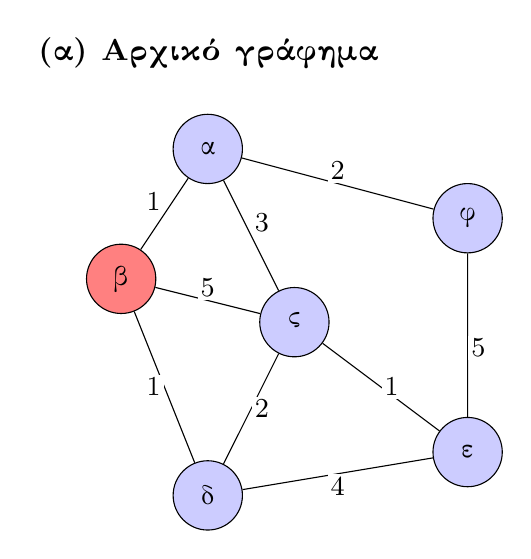
\begin{tikzpicture}[scale=1.1, every node/.style={transform shape}]
    % Κορυφές
    \node[vertex] (a) at (0,2) {a};
    \node[vertex, fill=red!50] (b) at (-1,0.5) {b};
    \node[vertex] (c) at (1,0) {c}; 
    \node[vertex] (d) at (0,-2) {d};
    \node[vertex] (e) at (3,-1.5) {e};
    \node[vertex] (f) at (3,1.2) {f};

    % Ακμές με βάρη
    \draw (a) -- (b) node[midway, above left, edge weight] {1};
    \draw (a) -- (c) node[midway, above right, edge weight] {3};
    \draw (a) -- (f) node[midway, above, edge weight] {2};
    \draw (b) -- (c) node[midway, above, edge weight] {5};
    \draw (b) -- (d) node[midway, left, edge weight] {1};
    \draw (c) -- (d) node[midway, right, edge weight] {2};
    \draw (c) -- (e) node[midway, right, edge weight] {1};
    \draw (e) -- (f) node[midway, below right, edge weight] {5};
    \draw (d) -- (e) node[midway, below, edge weight] {4};

    % Τίτλος γράφου
    \node[draw=none, fill=none, above=0.4cm of a, font=\bfseries] {(α) Αρχικό γράφημα};
    
\end{tikzpicture}
\end{minipage}
\hfill
\begin{minipage}{0.45\textwidth}
\centering
% Πίνακας d[] με κουτάκια μόνο στην κάτω γραμμή
\selectlanguage{english}

\begin{tabular}{ccccccc}
  & a & b & c & d & e & f \\
\cline{2-7}
$d[]$ & \multicolumn{1}{|c|}{1} & \multicolumn{1}{|c|}{0} & \multicolumn{1}{|c|}{5} & \multicolumn{1}{|c|}{1} & \multicolumn{1}{|c|}{$\infty$} & \multicolumn{1}{|c|}{$\infty$} \\
\cline{2-7}
\end{tabular}

\selectlanguage{greek}

\vspace{0.5em}

% Πίνακας γειτνίασης
\[
\begin{array}{c}
a \\ b \\ c \\ d \\ e \\ f
\end{array}
\;
\left[
\begin{array}{cccccc}
0 & 1 & 3 & \infty & \infty & 2 \\
\rowcolor{gray!25}
1 & 0 & 5 & 1 & \infty & \infty \\
3 & 5 & 0 & 2 & 1 & \infty \\
\infty & 1 & 2 & 0 & 4 & \infty \\
\infty & \infty & 1 & 4 & 0 & 5 \\
2 & \infty & \infty & \infty & 5 & 0
\end{array}
\right]
\]

\end{minipage}
\vspace{3cm}

\hfill
\begin{minipage}{0.45\textwidth}
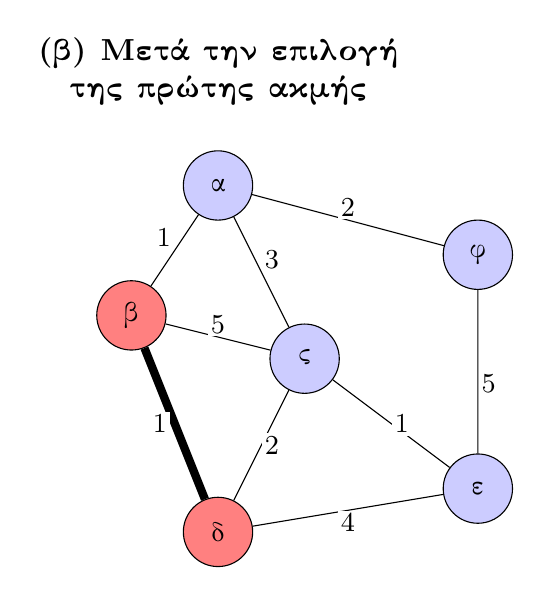
\begin{tikzpicture}[scale=1.1, every node/.style={transform shape}]
    % Κορυφές
    \node[vertex] (a) at (0,2) {a};
    \node[vertex, fill=red!50] (b) at (-1,0.5) {b};
    \node[vertex] (c) at (1,0) {c}; 
    \node[vertex, fill=red!50] (d) at (0,-2) {d};
    \node[vertex] (e) at (3,-1.5) {e};
    \node[vertex] (f) at (3,1.2) {f};

    % Ακμές με βάρη
    \draw (a) -- (b) node[midway, above left, edge weight] {1};
    \draw (a) -- (c) node[midway, above right, edge weight] {3};
    \draw (a) -- (f) node[midway, above, edge weight] {2};
    \draw (b) -- (c) node[midway, above, edge weight] {5};
    % <-- ΕΔΩ κάνουμε τη γραμμή πιο έντονη -->
    \draw [line width=3pt, color=black] (b) -- (d) node[midway, left, edge weight] {1};
    \draw (c) -- (d) node[midway, right, edge weight] {2};
    \draw (c) -- (e) node[midway, right, edge weight] {1};
    \draw (e) -- (f) node[midway, below right, edge weight] {5};
    \draw (d) -- (e) node[midway, below, edge weight] {4};

    % Τίτλος γράφου
 \node[draw=none, fill=none, above=0.4cm of a, font=\bfseries, align=center] 
{(β) Μετά την επιλογή \\ της πρώτης ακμής};

\end{tikzpicture}
\end{minipage}
\hfill
\begin{minipage}{0.45\textwidth}
\centering
% Πίνακας d[] με κουτάκια μόνο στην κάτω γραμμή
\selectlanguage{english}

\begin{tabular}{ccccccc}
  & a & b & c & d & e & f \\
\cline{2-7}
$d[]$ & \multicolumn{1}{|c|}{1} & \multicolumn{1}{|c|}{0} & \multicolumn{1}{|c|}{2} & \multicolumn{1}{|c|}{1} & \multicolumn{1}{|c|}{4} & \multicolumn{1}{|c|}{$\infty$} \\
\cline{2-7}
\end{tabular}

\selectlanguage{greek}

\vspace{0.5em}

% Πίνακας γειτνίασης
\[
\begin{array}{c}
a \\ b \\ c \\ d \\ e \\ f
\end{array}
\;
\left[
\begin{array}{cccccc}
0 & 1 & 3 & \infty & \infty & 2 \\
1 & 0 & 5 & 1 & \infty & \infty \\
3 & 5 & 0 & 2 & 1 & \infty \\
\rowcolor{gray!25}
\infty & 1 & 2 & 0 & 4 & \infty \\
\infty & \infty & 1 & 4 & 0 & 5 \\
2 & \infty & \infty & \infty & 5 & 0
\end{array}
\right]
\]
\end{minipage}
\vspace{3cm}


\hfill
\begin{minipage}{0.45\textwidth}
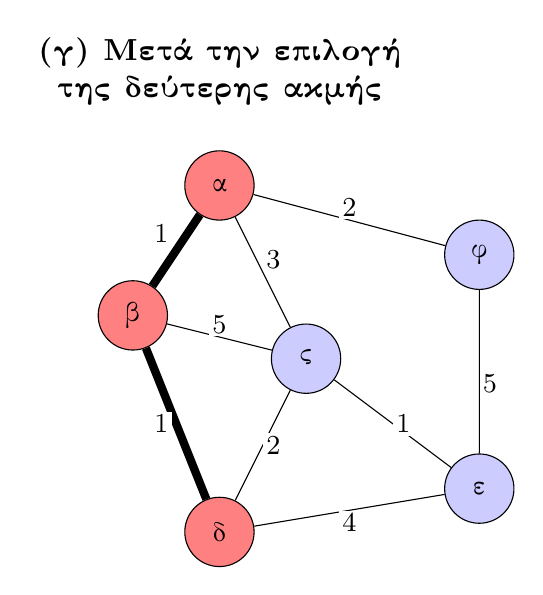
\begin{tikzpicture}[scale=1.1, every node/.style={transform shape}]
    % Κορυφές
    \node[vertex, fill=red!50] (a) at (0,2) {a};
    \node[vertex, fill=red!50] (b) at (-1,0.5) {b};
    \node[vertex] (c) at (1,0) {c}; 
    \node[vertex, fill=red!50] (d) at (0,-2) {d};
    \node[vertex] (e) at (3,-1.5) {e};
    \node[vertex] (f) at (3,1.2) {f};

    % Ακμές με βάρη
    \draw [line width=3pt, color=black] (a) -- (b) node[midway, above left, edge weight] {1};
    \draw (a) -- (c) node[midway, above right, edge weight] {3};
    \draw (a) -- (f) node[midway, above, edge weight] {2};
    \draw (b) -- (c) node[midway, above, edge weight] {5};
    % <-- ΕΔΩ κάνουμε τη γραμμή πιο έντονη -->
    \draw [line width=3pt, color=black] (b) -- (d) node[midway, left, edge weight] {1};
    \draw (c) -- (d) node[midway, right, edge weight] {2};
    \draw (c) -- (e) node[midway, right, edge weight] {1};
    \draw (e) -- (f) node[midway, below right, edge weight] {5};
    \draw (d) -- (e) node[midway, below, edge weight] {4};

    % Τίτλος γράφου
 \node[draw=none, fill=none, above=0.4cm of a, font=\bfseries, align=center] 
{(γ) Μετά την επιλογή \\ της δεύτερης ακμής};

\end{tikzpicture}
\end{minipage}
\hfill
\begin{minipage}{0.45\textwidth}
\centering
% Πίνακας d[] με κουτάκια μόνο στην κάτω γραμμή
\selectlanguage{english}

\begin{tabular}{ccccccc}
  & a & b & c & d & e & f \\
\cline{2-7}
$d[]$ & \multicolumn{1}{|c|}{1} & \multicolumn{1}{|c|}{0} & \multicolumn{1}{|c|}{2} & \multicolumn{1}{|c|}{1} & \multicolumn{1}{|c|}{4} & \multicolumn{1}{|c|}{2} \\
\cline{2-7}
\end{tabular}

\selectlanguage{greek}

\vspace{0.5em}


% Πίνακας γειτνίασης
\[
\begin{array}{c}
a \\ b \\ c \\ d \\ e \\ f
\end{array}
\;
\left[
\begin{array}{cccccc}
\rowcolor{gray!25}
0 & 1 & 3 & \infty & \infty & 2 \\
1 & 0 & 5 & 1 & \infty & \infty \\
3 & 5 & 0 & 2 & 1 & \infty \\
\infty & 1 & 2 & 0 & 4 & \infty \\
\infty & \infty & 1 & 4 & 0 & 5 \\
2 & \infty & \infty & \infty & 5 & 0
\end{array}
\right]
\]
\end{minipage}
\vspace{3cm}

\begin{figure}[ht]
\hfill
\begin{minipage}{0.45\textwidth}
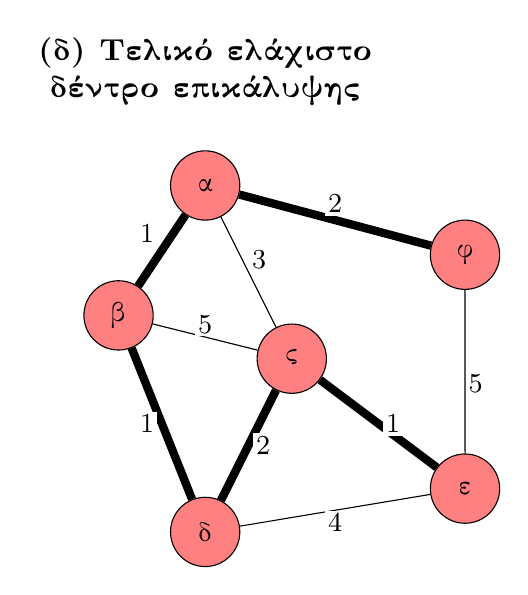
\begin{tikzpicture}[scale=1.1, every node/.style={transform shape}]
    % Κορυφές
    \node[vertex, fill=red!50] (a) at (0,2) {a};
    \node[vertex, fill=red!50] (b) at (-1,0.5) {b};
    \node[vertex, fill=red!50] (c) at (1,0) {c}; 
    \node[vertex, fill=red!50] (d) at (0,-2) {d};
    \node[vertex, fill=red!50] (e) at (3,-1.5) {e};
    \node[vertex, fill=red!50] (f) at (3,1.2) {f};

    % Ακμές με βάρη
    \draw [line width=3pt, color=black] (a) -- (b) node[midway, above left, edge weight] {1};
    \draw (a) -- (c) node[midway, above right, edge weight] {3};
    \draw [line width=3pt, color=black] (a) -- (f) node[midway, above, edge weight] {2};
    \draw (b) -- (c) node[midway, above, edge weight] {5};
    % <-- ΕΔΩ κάνουμε τη γραμμή πιο έντονη -->
    \draw [line width=3pt, color=black] (b) -- (d) node[midway, left, edge weight] {1};
    \draw [line width=3pt, color=black] (c) -- (d) node[midway, right, edge weight] {2};
    \draw [line width=3pt, color=black] (c) -- (e) node[midway, right, edge weight] {1};
    \draw (e) -- (f) node[midway, below right, edge weight] {5};
    \draw (d) -- (e) node[midway, below, edge weight] {4};

    % Τίτλος γράφου
 \node[draw=none, fill=none, above=0.4cm of a, font=\bfseries, align=center] 
{(δ) Τελικό ελάχιστο \\ δέντρο επικάλυψης};

\end{tikzpicture}
\end{minipage}
\hfill
\begin{minipage}{0.45\textwidth}
\centering
% Πίνακας d[] με κουτάκια μόνο στην κάτω γραμμή
\selectlanguage{english}

\begin{tabular}{ccccccc}
  & a & b & c & d & e & f \\
\cline{2-7}
$d[]$ & \multicolumn{1}{|c|}{1} & \multicolumn{1}{|c|}{0} & \multicolumn{1}{|c|}{2} & \multicolumn{1}{|c|}{1} & \multicolumn{1}{|c|}{1} & \multicolumn{1}{|c|}{2} \\
\cline{2-7}
\end{tabular}

\selectlanguage{greek}

\vspace{0.5em}

% Πίνακας γειτνίασης
\[
\begin{array}{c}
a \\ b \\ c \\ d \\ e \\ f
\end{array}
\;
\left[
\begin{array}{cccccc}
0 & 1 & 3 & \infty & \infty & 2 \\
1 & 0 & 5 & 1 & \infty & \infty \\
3 & 5 & 0 & 2 & 1 & \infty \\
\infty & 1 & 2 & 0 & 4 & \infty \\
\infty & \infty & 1 & 4 & 0 & 5 \\
2 & \infty & \infty & \infty & 5 & 0
\end{array}
\right]
\]
\vspace{1cm}
\end{minipage}

\vspace{0.3cm}
\noindent\rule{\textwidth}{0.2pt}

\caption{Ο αλγόριθμος του \foreignlanguage{english}{Prim} για το ελάχιστο δέντρο επικάλυψης. Το \foreignlanguage{english}{MST} έχει ρίζα την κορυφή b. Κατά τη διάρκεια κάθε επανάληψης, επιλέγεται η ακμή ελάχιστου κόστους που συνδέει μια κορυφή στο $V_T$ με μια κορυφή στο $V-V_T$ και η αντίστοιχη κορυφή προστίθεται στο $V_T$ (φαίνεται σκιασμένη στον πίνακα απόστασης $d$). Στη συνέχεια, οι τιμές $d[v]$ των κορυφών στο $V-V_T$ ενημερώνονται.}
\label{fig:graph5}
\end{figure}
\vspace{0.5cm}

\begin{figure}[ht]
\hfill

\centering
\begin{tabular}{p{1.2cm}ccccccccc}
    & & & & & & & & \makebox[0pt][c]{$\left|\frac{n}{p}\right|$} \\

\cline{2-9}
$d[1..n]$ 
  & \multicolumn{1}{|c|}{} 
  & \multicolumn{1}{|c|}{} 
  & \multicolumn{2}{|c|}{...}      
  & \multicolumn{1}{|c|}{} 
  & \multicolumn{2}{|c|}{...}      
  & \multicolumn{1}{|c|}{} \\      
\cline{2-9}
\end{tabular}
\quad ($a$)

\centering
\begin{tabular}{p{1.9cm}cccccccc}
  & & & & & & & & \\
\cline{2-9}
\raisebox{7\height}{\hspace{0.5cm}$A$}
  & \multicolumn{1}{|c|}{%
        \makebox[0pt][c]{\rotatebox{90}{==================}}%
        \rule{0pt}{100pt}
    }
& \multicolumn{1}{|c|}{%
        \makebox[0pt][c]{\rotatebox{90}{==================}}%
        \rule{0pt}{100pt}
    } 
& \multicolumn{2}{|c|}{%
    \raisebox{50pt}{\makebox[0pt][c]{...}}%
}

   
& \multicolumn{1}{|c|}{%
        \makebox[0pt][c]{\rotatebox{90}{==================}}%
        \rule{0pt}{100pt}
    } 
& \multicolumn{2}{|c|}{%
    \raisebox{50pt}{\makebox[0pt][c]{...}}%
}
    
& \multicolumn{1}{|c|}{%
        \makebox[0pt][c]{\rotatebox{90}{==================}}%
        \rule{0pt}{100pt}
    } \\
\cline{2-9}
\\[-2pt]
\hspace{-1cm}\foreignlanguage{english}{Processors}
  & \makebox[0pt][c]{0} & \makebox[0pt][c]{1}& \multicolumn{2}{c}{} & \makebox[0pt][c]{$i$} & \multicolumn{2}{c}{} & \makebox[0pt][c]{$p-1$}  \\

\end{tabular}
\begin{tikzpicture}[baseline=-0.5ex, xshift=3cm, yshift=-2.15cm]
  % Κάθετο διπλοβέλος, μετακινημένο προς τα πάνω
  \draw[<->] (0,4.6) -- (0,0.2);
  \node at (0.3,2.3) {$n$};
\end{tikzpicture}
\quad ($b$)


\vspace{0.3cm}
\noindent\rule{\textwidth}{0.2pt}

\caption{Η διαμέριση του πίνακα απόστασης $d$ και ο πίνακας γειτνίασης Α μεταξύ $p$ επεξεργαστών.}
\label{fig:graph6}
\end{figure}
\vspace{0.5cm}
 
\subsection{Παράλληλη Υλοποίηση}
Ο αλγόριθμος του \foreignlanguage{english}{Prim} είναι επαναληπτικός. Κάθε επανάληψη προσθέτει μια νέα κορυφή στο ελάχιστο δέντρο επικάλυψης. Δεδομένου ότι η τιμή του $d[v]$ για μια κορυφή $v$ μπορεί να αλλάζει κάθε φορά που προστίθεται μια νέα κορυφή $u$ στο $V_T$, είναι δύσκολο να επιλεγούν περισσότερες από μία κορυφές για να συμπεριληφθούν στο ελάχιστο δέντρο επικάλυψης. Για παράδειγμα, στο γράφημα του Σχήματος ~\ref{fig:graph5}, έπειτα από την επιλογή της κορυφής $b$, εάν και οι δύο κορυφές $d$ και $c$ επιλεγούν, το \foreignlanguage{english}{MST} δεν θα βρεθεί. Αυτό συμβαίνει γιατί, έπειτα από την επιλογή της κορυφής $d$, η τιμή της $d[c]$ ενημερώνεται από 5 σε 2. Επομένως, δεν είναι εύκολο να εκτελεστούν παράλληλα διαφορετικές επαναλήψεις του βρόχου $while$. Ωστόσο, κάθε επανάληψη μπορεί να εκτελεστεί παράλληλα ως εξής. 

Έστω $p$ ο αριθμός των επεξεργαστών και $n$ ο αριθμός των κορυφών στο γράφημα. Το σύνολο $V$ χωρίζεται σε $p$ υποσύνολα χρησιμοποιώντας την $block$ διαμέριση σε λωρίδες. Κάθε υποσύνολο έχει $\frac{n}{p}$ συνεχόμενες κορυφές και η εργασία που σχετίζεται με κάθε υποσύνολο ανατίθεται σε διαφορετικό επεξεργαστή. Έστω $V_i$ το υποσύνολο των κορυφών που έχουν ανατεθεί στον επεξεργαστή $P_i$ για $i = 0, 1, ..., p - 1$. Κάθε επεξεργαστής $P_i$ αποθηκεύει το τμήμα του πίνακα $d$ που αντιστοιχεί στο $V_i$ (δηλαδή, ο επεξεργαστής $P_i$ αποθηκεύει το $d[v]$ έτσι ώστε $v \in V_i$). Το Σχήμα ~\ref{fig:graph6}(a) απεικονίζει την διαμέριση. Κάθε επεξεργαστής $P_i$ υπολογίζει $d_i[u] = \min \{\, d_i[v] \mid v \in (V - V_T) \cap V_i \,\}$ κατά τη διάρκεια κάθε επανάληψης του βρόχου $while$. Το συνολικό ελάχιστο λαμβάνεται τότε για όλα τα $d_i[u]$ χρησιμοποιώντας την ένα-προς-όλους μετάδοση και αποθηκεύεται στον επεξεργαστή $P_0$. Ο επεξεργαστής $P_0$ διατηρεί τώρα τη νέα κορυφή $u$, η οποία θα εισαχθεί στο $V_T$. Ο επεξεργαστής $P_0$ μεταδίδει το $u$ σε όλους τους επεξεργαστές χρησιμοποιώντας την ένα-προς-όλους μετάδοση. Ο επεξεργαστής $P_i$ που είναι υπεύθυνος για την κορυφή $u$ σημειώνει το $u$ ότι ανήκει στο σύνολο $V_T$. Τέλος, κάθε επεξεργαστής ενημερώνει τις τιμές του $d[v]$ για τις τοπικές κορυφές του. 

Όταν μια νέα κορυφή $u$ εισέρχεται στο $V_T$, οι τιμές του $d[v]$ για το $v \in (V - V_T)$ πρέπει να ενημερωθούν. Ο επεξεργαστής που είναι υπεύθυνος για το $v$ πρέπει να γνωρίζει το βάρος της ακμής $(u, v)$. Επομένως, κάθε επεξεργαστής $P_i$ πρέπει να αποθηκεύει τις στήλες του πίνακα γειτνίασης με βάρη που αντιστοιχούν στο σύνολο $V_i$ των κορυφών που έχουν εκχωρηθεί σε αυτόν. Ο χώρος για την αποθήκευση του απαιτούμενου τμήματος του πίνακα γειτνίασης με βάρη σε κάθε επεξεργαστή είναι $\Theta\!\left(\frac{n^2}{p}\right)$.Το Σχήμα ~\ref{fig:graph6}(b) απεικονίζει τον διαμερισμό του πίνακα γειτνίασης με βάρη. Ο υπολογισμός που εκτελείται από έναν επεξεργαστή για την ελαχιστοποίηση και την ενημέρωση των τιμών του $d[v]$ κατά τη διάρκεια κάθε επανάληψης είναι $\Theta\!\left(\frac{n}{p}\right)$. Η επικοινωνία που εκτελείται σε κάθε επανάληψη οφείλεται στη μονού κόμβου συσσώρευση και στη μετάδοση ενός προς όλους.
\vspace{0.3cm}

\subsubsection*{Υπερκύβος}
Για έναν υπερκύβο με $p$-επεξεργαστές, η μια-προς-όλους μετάδοση μιας λέξης από έναν προς όλους απαιτεί χρόνο
$(t_s + t_w)$ $\log p$. Η εύρεση του συνολικού ελάχιστου μιας λέξης σε κάθε
επεξεργαστή απαιτεί τον ίδιο χρόνο. Έτσι, το συνολικό κόστος επικοινωνίας
κάθε επανάληψης είναι $\Theta(\log p)$. Ο παράλληλος χρόνος εκτέλεσης αυτής της διατύπωσης δίνεται από 
\[
T_p =
\overbrace{\Theta\!\left(\frac{n^2}{p}\right)}^{\text{υπολογισμός}}
+
\overbrace{\Theta(n \log p)}^{\text{επικοινωνία}}
\]
Δεδομένου ότι ο ακολουθιακός χρόνος εκτέλεσης είναι $W = \Theta(n^2)$, η επιτάχυνση και η αποδοτικότητα είναι οι εξής:
\[ S = \frac{\Theta(n^2)}{\Theta\!\left(\frac{n^2}{p}\right) + \Theta(n \log p)} \]
\begin{equation}
E = \frac{1}{1 + \Theta\!\left(\frac{p \log p}{n}\right)}
\label{eq:relation1}
\end{equation}
Από την Εξίσωση ~(\ref{eq:relation1}) βλέπουμε ότι για μια βέλτιστη ως προς το κόστος παράλληλη υλοποίηση, χρειαζόμαστε χρόνο \(\frac{p \log p}{n} = O(1)\). Έτσι, η υλοποίηση σε υπερκύβο του αλγορίθμου του foreignlanguage{english}{Prim} μπορεί να χρησιμοποιήσει μόνο \( p = O(n / \log n) \) επεξεργαστές. Επιπλέον, από την Εξίσωση ~(\ref{eq:relation1}), η συνάρτηση ισο-αποδοτικότητας λόγω
επικοινωνίας είναι $\Theta(p^2 \log^2 p)$. Δεδομένου ότι το $n$ πρέπει να αυξάνεται τουλάχιστον τόσο γρήγορα όσο το $p$ σε αυτή τη
υλοποίηση, η συνάρτηση ισο-αποδοτικότητας λόγω ταυτόχρονης εκτέλεσης είναι $\Theta(p^2)$. Έτσι, η συνολική
ισοαποδοτικότητα αυτής της υλοποίησης είναι $\Theta(p^2 \log^2 p)$.

\vspace{0.3cm}
\subsubsection*{Πλέγμα}
Για ένα πλέγμα επεξεργαστών $p$, η εύρεση ενός ολικού ελάχιστου και η εκτέλεση μιας μετάδοσης ενός προς όλους απαιτούν χρόνο $\Theta(\sqrt{p})$. Επομένως, ο παράλληλος χρόνος εκτέλεσης του αλγορίθμου \foreignlanguage{english}{Prim} είναι 
\begin{equation}
T_p = \overbrace{\Theta\!\left(\frac{n^2}{p}\right)}^{\text{υπολογισμός}}
+ \overbrace{\Theta(n \sqrt{p})}^{\text{επικοινωνία}}
\label{eq:relation2}
\end{equation}

Δεδομένου ότι ο ακολουθιακός χρόνος εκτέλεσης είναι W = Θ($n^2$), η επιτάχυνση και η αποδοτικότητα είναι οι εξής:
\[
S = \frac{\Theta(n^2)}{\Theta\!\left(\frac{n^2}{p}\right) + \Theta(n\sqrt{p})}
\]
\begin{equation}
E = \frac{1}{1 + \Theta\!\left(\frac{p^{1.5}}{n}\right)}
\label{eq:relation3}
\end{equation}
Στη Εξίσωση ~(\ref{eq:relation3}) βλέπουμε ότι για έναν αλγόριθμο βέλτιστου κόστους, $p^{1.5}/n$ = O(1). Επομένως, μόνο $O(n^{0.66})$ επεξεργαστές μπορούν να χρησιμοποιηθούν αποτελεσματικά. Επίσης από την Εξίσωση ~(\ref{eq:relation3}), η συνάρτηση ισοαποδοτικότητας λόγω επικοινωνίας είναι $\Theta(p^3)$. Αυτή είναι και η συνολική συνάρτηση ισοαποδοτικότητας. 
\vspace{0.5cm}

\section{Συντομότερες Διαδρομές από Μία Πηγή: Ο αλγόριθμος του \foreignlanguage{english}{Dijkstra}}

Για ένα γράφημα με βάρη $G = (V, E, w)$, το πρόβλημα \textbf{των συντομότερων διαδρομών από μία πηγή} είναι η εύρεση της συντομότερης διαδρομής από μια κορυφή $v \in V$ προς όλες τις άλλες κορυφές του $V$. \textbf{Μια συντομότερη διαδρομή} από $u$ προς $v$ είναι μια διαδρομή ελάχιστου βάρους. Ανάλογα με την εφαρμογή, τα βάρη των ακμών μπορεί να αντιπροσωπεύουν χρόνο, κόστος, ποινή, απώλεια ή οποιαδήποτε άλλη ποσότητα που αθροίζεται σωρρευτικά κατά μήκος μιας διαδρομής και πρέπει να ελαχιστοποιηθεί. Στην επόμενη ενότητα παρουσιάζουμε τον αλγόριθμο του \foreignlanguage{english}{Dijkstra}, ο οποίος λύνει το πρόβλημα των συντομότερων διαδρομών από μία πηγή τόσο σε κατευθυνόμενα όσο και σε μη κατευθυνόμενα γραφήματα με μη αρνητικά βάρη.

Ο αλγόριθμος του \foreignlanguage{english}{Dijkstra}, που βρίσκει τις συντομότερες διαδρομές από μία κορυφή $s$, είναι παρόμοιος με τον αλγόριθμο του \foreignlanguage{english}{Prim} για το ελάχιστο δέντρο επικάλυψης. Όπως και ο αλγόριθμος του \foreignlanguage{english}{Prim}, βρίσκει σταδιακά τις συντομότερες διαδρομές από το $s$ προς τις υπόλοιπες κορυφές του $G$. Είναι επίσης άπληστος. Δηλαδή, σε κάθε βήμα επιλέγει μια κορυφή που φαίνεται ότι βρίσκεται πλησιέστερα προς την πηγή. Ο Αλγόριθμος \ref{alg:dijkstra} δείχνει τον αλγόριθμο του \foreignlanguage{english}{Dijkstra}. Συγκρίνοντας αυτόν τον αλγόριθμο με τον αλγόριθμο του \foreignlanguage{english}{Prim} για το ελάχιστο δέντρο επικάλυψης, παρατηρούμε ότι οι δύο είναι σχεδόν ταυτόσημοι. Η βασική διαφορά είναι ότι, για κάθε κορυφή $u \in (V - V_T)$, ο αλγόριθμος του \foreignlanguage{english}{Dijkstra} αποθηκεύει $l[u]$, το ελάχιστο κόστος για να φτάσει στην κορυφή $u$ από την κορυφή $s$ χρησιμοποιώντας κορυφές στο $V_T$. O αλγόριθμος του \foreignlanguage{english}{Prim} αποθηκεύει $d[u]$, το κόστος της ακμής ελάχιστου κόστους που συνδέει μια κορυφή στο $V_T$ με την $u$. Ο χρόνος εκτέλεσης του αλγορίθμου του \foreignlanguage{english}{Dijkstra} είναι $\Theta(n^2)$.

\selectlanguage{english}

\begin{algorithm}[H]
\begin{algorithmic}[1]
\Procedure{DIJKSTRA\_SINGLE\_SOURCE\_SP}{$V, E, w, s$}
    \State $V_T \gets \{s\}$
    \State $l[s] \gets 0$
    \ForAll{$v \in (V - V_T)$}
        \If{edge $(s, v)$ exists}
            \State $l[v] \gets w(s, v)$
        \Else
            \State $l[v] \gets \infty$
        \EndIf
    \EndFor
    \While{$V_T \neq V$}
        \State find vertex $u$ such that $l[u] = \min\{l[v] \mid v \in (V - V_T)\}$
        \State $V_T \gets V_T \cup \{u\}$
        \ForAll{$v \in (V - V_T)$}
            \State $l[v] \gets \min\{l[v], l[u] + w(u, v)\}$
        \EndFor
    \EndWhile
\EndProcedure
\end{algorithmic}
\end{algorithm}

\selectlanguage{greek}

{\raggedright\refstepcounter{algorithm}\textbf{Αλγόριθμος \thealgorithm:} Ο σειριακός αλγόριθμος του \foreignlanguage{english}{Dijkstra} για τις συντομότερες διαδρομές από μία πηγή.\label{alg:dijkstra}\par}
\vspace{0.3cm}
 
\subsection{Παράλληλη Υλοποίηση}

Η παράλληλη υλοποίηση του αλγορίθμου του \foreignlanguage{english}{Dijkstra} για τις συντομότερες διαδρομές από μία πηγή είναι πολύ παρόμοια με την παράλληλη υλοποίηση του αλγορίθμου του \foreignlanguage{english}{Prim} για τα ελάχιστα δέντρα επικάλυψης (Ενότητα 2). Ο πίνακας γειτνίασης με βάρη διαιρείται χρησιμοποιώντας την $block-striped$ απεικόνιση. Κάθε ένας από τους $p$ επεξεργαστές ανατίθεται σε $n/p$ διαδοχικές στήλες του πίνακα γειτνίασης με βάρη και υπολογίζει $n/p$ τιμές του πίνακα $l$. Κατά τη διάρκεια κάθε επανάληψης, όλοι οι επεξεργαστές εκτελούν υπολογισμούς και επικοινωνία ανάλογη με εκείνη που εκτελείται στην παράλληλη υλοποίηση του αλγορίθμου του \foreignlanguage{english}{Prim}. 
\noindent
Ο Πίνακας~\ref{tab:prim_dijkstra_performance} παρουσιάζει τις μετρικές απόδοσης για τους αλγορίθμους του \foreignlanguage{english}{Prim} και του \foreignlanguage{english}{Dijkstra} σε συστήματα συνδεδεμένα ως δακτύλιος, πλέγμα και υπερκύβος. Σε όλες τις περιπτώσεις, ο παράλληλος χρόνος εκτέλεσης για μια βέλτιστη υλοποίηση ως προς το κόστος είναι επίσης ο ελάχιστος παράλληλος χρόνος εκτέλεσης που μπορεί να επιτευχθεί σε κάθε αρχιτεκτονική σε ασυμπτωτικούς όρους (Πρόβλημα 7.1).
\medskip
\begin{table}[ht]
\centering
\caption{Επιδόσεις των αλγορίθμων \foreignlanguage{english}{Prim} και \foreignlanguage{english}{Dijkstra} σε διαφορετικές αρχιτεκτονικές.}
\label{tab:prim_dijkstra_performance}
\begingroup
\setlength{\tabcolsep}{2.5pt}% slightly tighter column separation to avoid overfull
\footnotesize
\begin{tabular}{>{\raggedright\arraybackslash}p{2.4cm} >{\raggedright\arraybackslash}p{5.2cm} >{\hspace{-16mm}\centering\arraybackslash}p{2.8cm} >{\raggedright\arraybackslash}p{4.0cm}}
\toprule
{\scriptsize\textbf{Αρχιτεκτονική}} & {\scriptsize\textbf{\shortstack{Μέγιστος αριθμός \\ επεξεργαστών για $E=\Theta(1)$}}} & {\scriptsize\textbf{\shortstack{Αντίστοιχος \\ παράλληλος χρόνος}}} & {\scriptsize\textbf{\shortstack{Συνάρτηση \\ ισοαποδοτικότητας}}} \\
\midrule
Δακτύλιος & $\Theta(\sqrt{n})$ & $\Theta(n^{1.5})$ & $\Theta(p^{4})$ \\
Πλέγμα & $\Theta(n^{0.66})$ & $\Theta(n^{1.33})$ & $\Theta(p^{3})$ \\
Υπερκύβος & $\Theta\left(\dfrac{n}{\log n}\right)$ & $\Theta(n\log n)$ & $\Theta\big(p^{2}\log^{2} p\big)$ \\
\bottomrule
\end{tabular}
\endgroup
\end{table}
 
% Προσθήκη μεταφρασμένου τμήματος (ελληνικά)
\subsubsection{\foreignlanguage{english}{API}/Σύστημα μεταβίβασης μηνυμάτων}

Το \foreignlanguage{english}{API} μεταβίβασης μηνυμάτων πρέπει να είναι διαθέσιμο σε όλα τα συστήματα στα οποία
υλοποιείται και θα πρέπει να είναι όσο το δυνατόν πιο απλό και ευθύ, προτιμητέα να
υποστηρίζει συλλογικές λειτουργίες. Το \foreignlanguage{english}{MPI} καλύπτει αυτές τις απαιτήσεις, επομένως δεν απαιτείται σοβαρή εξέταση εναλλακτικών κατά την επιλογή του. Η υλοποίηση του \foreignlanguage{english}{MPI} είναι δωρεάν, εύκολα διαθέσιμη, και παρέχει συνδέσεις (\foreignlanguage{english}{bindings}) για τη γλώσσα $C$ που είναι ευρέως γνωστή.
\vspace{0.2cm}


\subsubsection{\foreignlanguage{english}{API}/Σύστημα κοινής διεύθυνσης}

Το επιλεγμένο \foreignlanguage{english}{API} κοινής διεύθυνσης πρέπει να επιτρέπει μεγάλο έλεγχο πάνω στις εργασίες
που εκτελούνται ταυτόχρονα. Πρέπει επίσης να παρέχεται δωρεάν. Το \foreignlanguage{english}{OpenMP} παρέχει ένα
επίπεδο πάνω από τις εγγενείς νηματικές (\foreignlanguage{english}{thread}) λειτουργίες για τη διευκόλυνση
διαφόρων εργασιών σχετικών με νήματα. Χρησιμοποιώντας τις οδηγίες που παρέχει το \foreignlanguage{english}{OpenMP},
ο προγραμματιστής δεν χρειάζεται να εκτελέσει την εργασία αρχικοποίησης του αντικειμένου
ιδιοτήτων, να ορίσει παραμέτρους για το νήμα και να διαιρέσει τον χώρο επανάληψης. Αυτή η
δυνατότητα είναι ιδιαίτερα χρήσιμη όταν το υποκείμενο πρόβλημα έχει στατικό ή τακτικό
διάγραμμα εργασιών. Στο πλαίσιο διαφόρων εφαρμογών, έχει αποδειχθεί ότι το κόστος που
σχετίζεται με την αυτόματη δημιουργία κώδικα νημάτων από αυτές τις οδηγίες είναι
ελάχιστο.
\vspace{0.2cm}

\subsubsection{Γλώσσα}

Επιλέγεται τη γλώσσα $C$ λόγω της διαθεσιμότητας μιας σχετικά σταθερής υλοποίησης του \foreignlanguage{english}{MPI}
για μεταβίβαση μηνυμάτων και της βιβλιοθήκης για \foreignlanguage{english}{OpenMP}.
\vspace{0.2cm}

\subsubsection{Περιβάλλον συστήματος}

Η σειριακή υλοποίηση του αλγορίθμου του \foreignlanguage{english}{Dijkstra}, η υλοποίηση του αλγορίθμου του \foreignlanguage{english}{Dijkstra} με \foreignlanguage{english}{MPI} και η υλοποίηση του αλγορίθμου του \foreignlanguage{english}{Dijkstra} με
\foreignlanguage{english}{OpenMP}, και οι τρεις υλοποιήσεις εκτελούνται στο σύστημα του \foreignlanguage{english}{Minnesota Supercomputing
Institute (MSI)}.
\vspace{0.2cm}

\subsection{Δεδομένα δοκιμών}

Αφού ορίστηκαν οι τεχνολογίες που θα χρησιμοποιηθούν, χρειάζεται ένα πρόγραμμα σε \foreignlanguage{english}{JAVA} για
τη δημιουργία δοκιμαστικών δεδομένων. Το πρόγραμμα αυτό παράγει έναν δισδιάστατο πίνακα
με τυχαίους αριθμούς στο διάστημα 1 έως 15, που αντιπροσωπεύει το γράφο εισόδου για τον
αλγόριθμο του \foreignlanguage{english}{Dijkstra}. Τα βάρη δημιουργούνται με τη συνάρτηση \foreignlanguage{english}{Random} της \foreignlanguage{english}{JAVA}. Έστω
$G$ ένας δισδιάστατος πίνακας, όπου $G[i][j]$ αντιπροσωπεύει το βάρος από την κορυφή $i$ προς
την κορυφή $j$. Εάν δεν υπάρχει άμεση σύνδεση, το βάρος ορίζεται σε 9999999, αλλιώς είναι
ένας τυχαίος αριθμός μεταξύ 1 και 15. Όταν $i = j$, πρόκειται για την ίδια κορυφή, οπότε
ορίζουμε $G[i][j] = 0$ σε αυτή την περίπτωση. Τα βάρη παράγονται τυχαία, και η υπολογιζόμενη
απόσταση δεν θα είναι πολύ μεγάλη. Αυτό δεν επηρεάζει τους πειραματικούς μας στόχους,
εφόσον χρειάζομαι μόνο τα αποτελέσματα από διαφορετικά προγράμματα που χρησιμοποιούν τα
ίδια δεδομένα. Θα τρέξω το ίδιο σύνολο δεδομένων στη σειριακή υλοποίηση του αλγορίθμου του \foreignlanguage{english}{Dijkstra}, στην υλοποίηση του αλγορίθμου του \foreignlanguage{english}{Dijkstra} με \foreignlanguage{english}{MPI} και στην υλοποίηση του αλγορίθμου του \foreignlanguage{english}{Dijkstra} με
\foreignlanguage{english}{OpenMP} για να συγκρίνω τους χρόνους εκτέλεσης. Συνολικά
χρησιμοποιούνται έξι σύνολα δεδομένων ως πίνακες γειτνίασης. Αυτό σημαίνει για γράφους με 8, 64, 256,
512, 1024 και 2048 κορυφές. Ακολουθεί ένα παράδειγμα για τη μήτρα των 8 κορυφών.
\vspace{0.3cm}
\[
    \begingroup
    \setlength{\arraycolsep}{8pt}% horizontal gap between columns (default ~5pt)
    \renewcommand{\arraystretch}{2}% vertical stretch (default 1)
    \begin{array}{cccccccc}
        0 & 2 & 9999999 & 3 & 4 & 3 & 9999999 & 3 \\
        2 & 0 & 8 & 8 & 9 & 9999999 & 7 & 7 \\
        9999999 & 8 & 0 & 6 & 7 & 9999999 & 9999999 & 2 \\
        3 & 8 & 6 & 0 & 7 & 3 & 9 & 7 \\
        4 & 9 & 7 & 7 & 0 & 9999999 & 9999999 & 4 \\
        3 & 9999999 & 9999999 & 3 & 9999999 & 0 & 8 & 3 \\
        9999999 & 7 & 9999999 & 9 & 9999999 & 8 & 0 & 9999999 \\
        3 & 7 & 2 & 7 & 4 & 3 & 9999999 & 0 \\
    \end{array}
    \endgroup
\]
\vspace{0.3cm}

\subsection{Αλγόριθμος}
Στην παρακάτω ενότητα δίνονται λεπτομέρειες σχετικά με το πώς υλοποιήθηκε ο αλγόριθμος. Ο πλήρης πηγαίος κώδικας για τις περιγραφόμενες υλοποιήσεις βρίσκεται στο Παράρτημα Α. Εδώ παρέχεται ψευδοκώδικας που περιγράφει τις υλοποιήσεις σε απλοποιημένη μορφή.
\vspace{0.2cm}

\subsubsection{Υλοποίηση του αλγορίθμου του \foreignlanguage{english}{Dijkstra} με \foreignlanguage{english}{MPI}}
Η υλοποίηση του αλγορίθμου, σε απλοποιημένη μορφή σύμφωνα με τον ψευδοκώδικα, παρουσιάζεται παρακάτω.

\selectlanguage{english}
\begin{algorithm}[H]
\begin{algorithmic}[1]
\Procedure{DIJKSTRA\_SINGLE\_SOURCE\_SP\_MPI}{$V, E, wgt, lengths, s$}
    \State initialize local and global data structures
    \ForAll{$v \in V$}
        \State set $lminpair[0]$: local min distance
        \State set $lminpair[1]$: corresponding vertex
    \EndFor
    \While{not all vertices processed}
        \State for vertices in each processor find a vertex $u$ with the smallest distance from the source $s$
        \State perform $\mathrm{MPI\_Allreduce}$ to obtain the global minimum across processors
        \State get the global minimum vertex $u$ and mark it as processed
        \ForAll{$v \in \text{nlocals}$} \Comment{nlocals = number of vertices stored locally}
            \State $lengths[v] \gets \min\{lengths[v], udist + wgt[u* nlocal + v]\}$
        \EndFor
    \EndWhile
\EndProcedure
\end{algorithmic}
\end{algorithm}

\selectlanguage{greek}

{\raggedright\refstepcounter{algorithm}\textbf{Αλγόριθμος \thealgorithm:} Ο αλγόριθμος του \foreignlanguage{english}{Dijkstra} με \foreignlanguage{english}{MPI} για τις συντομότερες διαδρομές από μία πηγή.\label{alg:dijkstra2}\par}
\vspace{0.3cm}

Ο βασικός υπολογιστικός βρόχος του παράλληλου αλγορίθμου του \foreignlanguage{english}{Dijkstra} για τις συντομότερες διαδρομές από μία πηγή εκτελεί τρία βήματα. Πρώτον, κάθε διεργασία εντοπίζει την τοπικά αποθηκευμένη κορυφή στο $V_o$ με τη μικρότερη απόσταση από την πηγή. Έπειτα, οι διεργασίες καθορίζουν την κορυφή με τη μικρότερη απόσταση και την προσθέτουν στο $V_c$. Τρίτον, κάθε διεργασία ενημερώνει τον πίνακα αποστάσεων ώστε να ληφθεί υπόψη ότι στο $V_c$ έχουν προστεθεί νέες κορυφές.

Το πρώτο βήμα είναι η σάρωση των τοπικών κορυφών του $V_o$ για να βρεθεί η κορυφή $v$ με τη μικρότερη τοπική απόσταση $[v]$. Το αποτέλεσμα του υπολογισμού αποθηκεύεται στον πίνακα \texttt{$lminpair$}. Συγκεκριμένα, ο \texttt{$lminpair[0]$} αποθηκεύει την απόσταση μεταξύ των κορυφών και ο \texttt{$lminpair[1]$} αποθηκεύει τις ίδιες τις κορυφές. Ακολουθώντας τα παρακάτω βήματα θα γίνει κατανοητό γιατί θα πρέπει να χρησιμοποιηθεί αυτή η λύση αποθήκευσης. Το επόμενο βήμα είναι ο προσδιορισμός της κορυφής με τη μικρότερη συνολική απόσταση προς την πηγή, το οποίο γίνεται ελαχιστοποιώντας την τιμή που περιέχεται στο \texttt{$lminpair[0]$}.

Ωστόσο, πέρα από την ίδια την ελάχιστη απόσταση, χρειάζεται και ο δείκτης (η ταυτότητα) της κορυφής που επιτυγχάνει αυτή την απόσταση. Γι' αυτό η κατάλληλη λειτουργία μείωσης είναι η \texttt{$MPI\_MINLOC$}, η οποία επιστρέφει την ελάχιστη τιμή και τον δείκτη που αντιστοιχεί στην ελάχιστη αυτή τιμή. Εξαιτίας της \texttt{$MPI\_MINLOC$} χρησιμοποιούμε πίνακα δύο στοιχείων \texttt{$lminpair$} για να αποθηκεύσουμε την απόσταση και την κορυφή που την επιτυγχάνει. Επιπλέον, όλες οι διεργασίες χρειάζονται το αποτέλεσμα της διαδικασία ανάκτησης δεδομένων για να εκτελέσουν το τρίτο βήμα, γι' αυτό χρησιμοποιούμε την \texttt{$MPI\_Allreduce$} για να πραγματοποιήσουμε τη μείωση. Το αποτέλεσμα της μείωσης επιστρέφεται στον πίνακα \texttt{$gminpair$}. Το τρίτο και τελευταίο βήμα κάθε επανάληψης εκτελείται σαρώνοντας τις τοπικές κορυφές που ανήκουν στο $V_o$ και ενημερώνοντας, για κάθε τοπική κορυφή $v$, την ελάχιστη απόσταση μεταξύ αυτής και της κορυφής-πηγής.

Στο πρόγραμμα \foreignlanguage{english}{MPI}, γίνεται ανάθεση σε κάθε επεξεργαστή $n/p$ διαδοχικές στήλες του πίνακα $W$ και χρησιμοποιείται η μείωση \texttt{$MPI\_MINLOC$} για να επιλεχθεί η κορυφή $v$ που θα συμπεριληφθεί στο $V_c$ σε κάθε επανάληψη. Αξίζει να σημειωθεί ότι ο δείκτης που επιστρέφει η \texttt{$MPI\_MINLOC$} σε συγκρίσεις όπως $(a,i)$ και $(a,j)$ είναι ο μικρότερος δείκτης όταν οι τιμές είναι ίδιες. Επομένως, μεταξύ των κορυφών που έχουν την ίδια ελάχιστη απόσταση προς την πηγή, προτιμώνται οι κορυφές με τον μικρότερο δείκτη. Αυτό μπορεί να οδηγήσει σε ανισορροπία φόρτου, αφού οι κορυφές που αποθηκεύονται σε διεργασίες με μικρότερους δείκτες τείνουν να περιλαμβάνονται πρώτες στο $V_c$ σε σχέση με αυτές που βρίσκονται σε διεργασίες με μεγαλύτερους δείκτες (ειδικά όταν πολλές κορυφές στο $V_o$ έχουν την ίδια μικρή απόσταση προς την πηγή). Συνεπώς, στις διεργασίες με μεγαλύτερους δείκτες το διαμορφωμένο μέγεθος του $V_o$ θα είναι μεγαλύτερο και ο συνολικός χρόνος εκτέλεσης μπορεί να κυριαρχείται από αυτές.

Μια λύση σε αυτό το πρόβλημα είναι η κυκλική κατανομή των στηλών του $W$. Αυτή η διαδικασία κατανομής συγκεντρώνει όλες τις $p$ κορυφές, ξεκινώντας από την κορυφή $i$. Σε αυτό το πλαίσιο, κάθε διεργασία εξακολουθεί να αναθέτει $n/p$ κορυφές αλλά οι δείκτες τους καλύπτουν σχεδόν ολόκληρο το γράφημα. Έτσι, η \texttt{$MPI\_MINLOC$} θα ευνοεί συστηματικά κορυφές με μικρότερους δείκτες και δεν θα προκαλείται ανισορροπία φόρτου [2].

\subsubsection{Υλοποίηση του αλγορίθμου του \foreignlanguage{english}{Dijkstra} με \foreignlanguage{english}{OpenMP}}

Οι περισσότερες δομές του \foreignlanguage{english}{OpenMP} εφαρμόζονται σε ένα δομημένο μπλοκ, δηλαδή σε ένα μπλοκ μιας ή περισσότερων εντολών με ένα σημείο εισόδου στην κορυφή και ένα σημείο εξόδου στο κάτω μέρος. Καθίσταται εφικτός ο εντοπισμός των υπολογιστικά εντατικών βρόχων στον σειριακό αλγόριθμο του \foreignlanguage{english}{Dijkstra} και οι επαναλήψεις του βρόχου γίνονται ανεξάρτητες, ενώ στη συνέχεια μπορεί να γίνει η τοποθέτηση των κατάλληλων οδηγιών του \foreignlanguage{english}{OpenMP} και να γίνουν δοκιμές.

\selectlanguage{english}
\begin{algorithm}[H]
\begin{algorithmic}[1]
\Procedure{DIJKSTRA\_SP\_OMP}{$V, E, w, distances, s$}
    \State begin
    \While{not all vertices processed}
        \State $\#\text{pragma omp parallel private}$
        \State $\text{shared}()$
        \State \texttt{omp\_get\_thread\_num()}
        \State \texttt{omp\_get\_num\_threads()}
        \State Each thread finds the min distance $u$ unconnected vertex inner
        \State $\#\text{pragma omp critical}$ \quad // update overall min
        \State $\#\text{pragma omp barrier}$
        \State $\#\text{pragma omp single}$ \quad // mark new vertex as done
        \ForAll{$v$ in each thread}
            \State $distances[v] \gets \min\{distances[v], distances[u] + w[u][v]\}$
        \EndFor
    \EndWhile
\EndProcedure
\end{algorithmic}
\end{algorithm}

\selectlanguage{greek}

{\raggedright\refstepcounter{algorithm}\textbf{Αλγόριθμος \thealgorithm:} Ο αλγόριθμος του \foreignlanguage{english}{Dijkstra} με \foreignlanguage{english}{OpenMP} για τις συντομότερες διαδρομές από μία πηγή.\label{alg:dijkstra3}\par}
\vspace{0.3cm}

Όπως δείχνει ο ψευδοκώδικας, η υλοποίηση του αλγορίθμου  \foreignlanguage{english}{Dijkstra} με \foreignlanguage{english}{OpenMP} είναι πολύ παρόμοια με τη σειριακή. 
Σε σύγκριση με την υλοποίηση με \foreignlanguage{english}{MPI}, η υλοποίηση με \foreignlanguage{english}{OpenMP} απαιτεί λιγότερες γραμμές κώδικα.
Η συνάρτηση \texttt{$omp\_set\_num\_threads$} ορίζει τον προεπιλεγμένο αριθμό νημάτων που θα δημιουργηθούν όταν συναντηθεί η επόμενη οδηγία \texttt{$parallel$}. Χρησιμοποιούμε αυτή τη συνάρτηση στη συνάρτηση \texttt{$main$}.
Η \texttt{$omp\_get\_num\_threads$} επιστρέφει τον αριθμό των νημάτων που συμμετέχουν σε μια ομάδα. Η \texttt{$omp\_get\_thread\_num$} επιστρέφει ένα μοναδικό αναγνωριστικό για κάθε νήμα στην ομάδα. Αυτός ο ακέραιος παίρνει τιμές από $0$ έως \texttt{$omp\_get\_num\_threads()-1$}.
Η οδηγία \texttt{$critical$} διασφαλίζει ότι, σε κάθε χρονική στιγμή κατά την εκτέλεση, μόνο ένα νήμα βρίσκεται μέσα σε μια κρίσιμη ενότητα προσδιορισμένη με ένα συγκεκριμένο όνομα.
Η \foreignlanguage{english}{OpenMP} παρέχει την οδηγία \texttt{$critical$} για την υλοποίηση κρίσιμων περιοχών. Μια κρίσιμη περιοχή επιτρέπει σε διαφορετικά νήματα να εκτελούν διαφορετικό κώδικα ενώ είναι προστατευμένα μεταξύ τους.
Το \texttt{$barrier$} είναι μία από τις πιο συχνά χρησιμοποιούμενες πρωτόγονες λειτουργίες συγχρονισμού. Η \foreignlanguage{english}{OpenMP} παρέχει την οδηγία \texttt{$barrier$}. Όταν η εκτέλεση συναντήσει αυτή την οδηγία, όλα τα νήματα της ομάδας περιμένουν μέχρι να φτάσουν τα υπόλοιπα και στη συνέχεια συνεχίζουν.
Η οδηγία \texttt{$single$} προσδιορίζει ένα δομημένο μπλοκ που εκτελείται από ένα μόνο νήμα. Κατά την είσοδο στο μπλοκ \texttt{$single$}, το πρώτο νήμα εισέρχεται και όλα τα υπόλοιπα νήματα προχωρούν μέχρι το τέλος του μπλοκ [2].
\vspace{0.5cm}

\section{Αποτελέσματα Υλοποίησης και Ανάλυση}

Ο Πίνακας 1 περιέχει όλα τα βασικά αποτελέσματα από την σειριακή εκτέλεση του αλγορίθμου του \foreignlanguage{english}{Dijkstra}, τα \foreignlanguage{english}{MPI} και \foreignlanguage{english}{OpenMP} προγράμματα. Ο κώδικας εκτελέστηκε στο ίδιο περιβάλλον συστήματος και τα δεδομένα εισόδου δημιουργήθηκαν με τη συνάρτηση \texttt{$Random$}. Στην παρούσα εργασία χρησιμοποιούνται συνολικά έξι σύνολα δεδομένων για την είσοδο του πίνακα γειτνίασης. Συγκεκριμένα, για το γράφο χρησιμοποιούνται 8 κορυφές, 64 κορυφές, 256 κορυφές, 512 κορυφές, 1024 κορυφές και 2048 κορυφές. Μετά την εκτέλεση του κώδικα, λαμβάνονται τα αποτελέσματα ως διάρκεια σε δευτερόλεπτα. Για τους παράλληλους υπολογισμούς με \foreignlanguage{english}{OpenMP} και \foreignlanguage{english}{MPI}, χρησιμοποιήθηκαν 2, 4, 8, 16, 32, 64, 128, 256 και 512 επεξεργαστές (ο αριθμός των κορυφών πρέπει να είναι μεγαλύτερος από τον αριθμό των επεξεργαστών) για την εκτέλεση του κώδικα.
\vspace{0.3cm}

\begin{table}[H]
\centering
\caption{Χρόνος εκτέλεσης σε δευτερόλεπτα και των τριών υλοποιήσεων}
\label{tab:dijkstra_performance}

\selectlanguage{english}
\resizebox{0.95\textwidth}{!}{%
\begin{tabular}{|l|c|c|c|c|c|c|}
\hline
 & 8 vertices & 64 vertices & 256 vertices & 512 vertices & 1024 vertices & 2048 vertices \\
\hline
Seq & 0.0035 & 0.0029 & 0.0099 & 0.1162 & 0.3568 & 0.9965 \\
\hline
OpenMP2 & 0.0003 & 0.0015 & 0.0093 & 0.0651 & 0.2493 & 0.8583 \\
\hline
OpenMP4 & 0.0003 & 0.0016 & 0.0109 & 0.0635 & 0.2488 & 0.7933 \\
\hline
OpenMP8 & 0.0007 & 0.8831 & 0.0140 & 0.0854 & 0.2807 & 0.9432 \\
\hline
OpenMP16 & & 0.0574 & 0.0233 & 0.2736 & 0.6794 & 1.7490 \\
\hline
OpenMP32 & & 0.0640 & 0.1186 & 0.5117 & 1.3014 & 2.8708 \\
\hline
OpenMP64 & & 0.0864 & 0.2030 & 0.7614 & 1.7558 & 3.5983 \\
\hline
OpenMP128 & & & 0.3302 & 1.3960 & 2.8929 & 5.9080 \\
\hline
OpenMP256 & & & 0.9902 & 2.7855 & 5.3655 & 10.5335 \\
\hline
OpenMP512 & & & & 6.1405 & 10.6755 & 20.9920 \\
\hline
MPI2 & 0.0246 & 0.0178 & 0.0287 & 0.1137 & 0.1316 & 0.5040 \\
\hline
MPI4 & 0.0353 & 0.0210 & 0.0218 & 0.0413 & 0.1281 & 0.4723 \\
\hline
MPI8 & 0.0144 & 0.0164 & 0.0264 & 0.0440 & 0.1324 & 1.3663 \\
\hline
MPI16 & & 0.0264 & 0.0453 & 0.1010 & 0.2055 & 3.3525 \\
\hline
MPI32 & & 10.8733 & 1.2415 & 56.9774 & 3.9622 & 21.4067 \\
\hline
MPI64 & & 27.2983 & 3.1004 & 67.9168 & 7.1446 & 41.7286 \\
\hline
MPI128 & & & 7.3566 & 19.8329 & 17.9661 & 119.9792 \\
\hline
MPI256 & & & 18.8646 & 32.8870 & 44.8353 & 343.0892 \\
\hline
MPI512 & & & & 488.7678 & 1733.9085 & 2399.9986 \\
\hline
\end{tabular}%
}
\end{table}

\vspace{0.3cm}

\begin{table}[H]
\centering
\caption{Ο καλύτερος χρόνος εκτέλεσης σε δευτερόλεπτα και των τριών υλοποιήσεων (οι αριθμοί στις παρενθέσεις δείχνουν το πλήθος των νημάτων/επεξεργαστών}
\label{tab:best_dijkstra_performance}

\selectlanguage{english}
\resizebox{0.95\textwidth}{!}{%
\begin{tabular}{|l|c|c|c|c|c|c|}
\hline
 & 8 vertices & 64 vertices & 256 vertices & 512 vertices & 1024 vertices & 2048 vertices \\
\hline
Seq & 0.0035 & 0.0029 & 0.0099 & 0.1162 & 0.3568 & 0.9965 \\
\hline
OpenMP & 0.0003(2) & 0.0015(2) & 0.0093(2) & 0.0635(4) & 0.2488(4) & 0.7933(4) \\
\hline
MPI & 0.0144(8) & 0.0164(8) & 0.0218(4) & 0.0413(4) & 0.1281(4) & 0.4723(4) \\
\hline
\end{tabular}%
}
\end{table}
\vspace{0.3cm}


\begin{figure}[H]
\centering
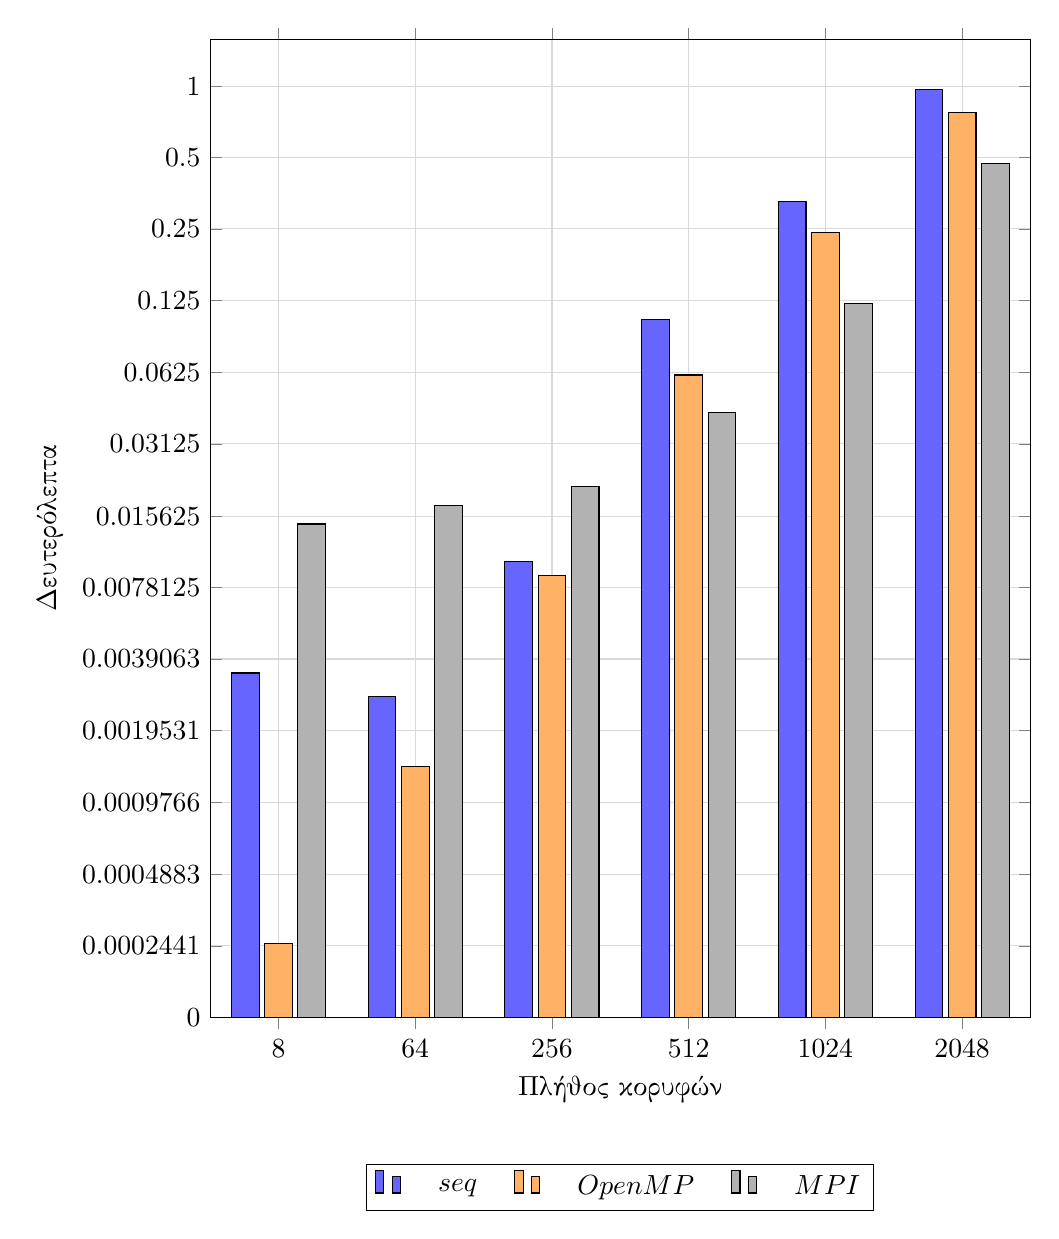
\begin{tikzpicture}
\begin{axis}[
    width=12cm,
    height=14cm,
    xlabel=Πλήθος κορυφών,
    ylabel=Δευτερόλεπτα,
    ybar,
    legend columns=3,
    legend style={at={(0.5,-0.15)}, anchor=north, column sep=0.4cm},
    bar width=10pt,
    x tick label style={rotate=0},
    xtick={1,2,3,4,5,6},
    xticklabels={8, 64, 256, 512, 1024, 2048},
    ytick={0, 0.077, 0.154, 0.231, 0.308, 0.385, 0.462, 0.538, 0.616, 0.693, 0.770, 0.847, 0.924, 1.0},
    yticklabels={0, 0.0002441, 0.0004883, 0.0009766, 0.0019531, 0.0039063, 0.0078125, 0.015625, 0.03125, 0.0625, 0.125, 0.25, 0.5, 1},
    grid=major,
    grid style={gray!30},
    ymin=0,
    ymax=1.05
]

\addplot[fill=blue!60, draw=black] coordinates {
    (1, 0.370) (2, 0.345) (3, 0.490) (4, 0.750) (5, 0.876) (6, 0.997)
};
\addlegendentry{$seq$}

\addplot[fill=orange!60, draw=black] coordinates {
    (1, 0.080) (2, 0.270) (3, 0.475) (4, 0.690) (5, 0.843) (6, 0.972)
};
\addlegendentry{$OpenMP$}

\addplot[fill=gray!60, draw=black] coordinates {
    (1, 0.530) (2, 0.550) (3, 0.570) (4, 0.650) (5, 0.767) (6, 0.917)
};
\addlegendentry{$MPI$}

\end{axis}
\end{tikzpicture}
\caption{Ο καλύτερος χρόνος εκτέλεσης για κάθε υλοποίηση σε διαφορετικά σύνολα δεδομένων}
\label{fig:execution_times}
\end{figure}

% Τέλος προσθήκης
\clearpage
\selectlanguage{english}
\printbibliography[
    title={\selectlanguage{greek}Βιβλιογραφία\selectlanguage{english}}
]
\selectlanguage{greek}
\addcontentsline{toc}{section}{Βιβλιογραφία}
\end{document}
